\documentclass[11pt]{report}
\usepackage{fullpage}
\usepackage{graphicx}
\usepackage{float}
\restylefloat{table}
\usepackage{url}
\begin{document}
\title{Developing a tool for teachers to increase awareness and understanding of Autism}
\author{Ashley Peacock}
\maketitle

\textbf{Abstract}\\
--add this when i'm finished 

\begin{quote}
"if you deal with 'challenging behaviours' in autism, do not focus on the iceberg; do understand the underlying causes of the behaviours and try to develop an approach not based on symptoms but on prevention. Challenging behaviours are caused by problems of communication, social understanding, by different imagination, by sensory problems...Therefore try to understand autism 'from within'. It is easier said than done, because it requires an enormous effort of imagination: we need t learn to put ourselves in the brains of autistic people and then we will understand better through their eyes the obstacles in their attempts to survive among us" - Theo Peeters \cite{olgab}
\end{quote}

\tableofcontents

\chapter{Overview}

The projected started by firstly creating and considering various project proposals that may benefit people with ADHD or Autism. Following this, research and feedback aided the selection of the project an "Autism Simulator" whereby the user plays as a child with Autism and gets to experience some of the difficulties, specifically sensory related difficulties through their eyes. Consultation with the Learning and Adaptive Environment Research(LAER lab) in addition to interviews with people on the Autistic spectrum, professionals and school teachers further solidified this selection and gave indication of the challenges faced as to inform design choices and goal selection. A prototype of the simulator was then created using a Game Engine for speedy development and the project was evaluated by the LAER group with an additional evaluation in the form of an on-line survey where participants were able to view a video demo of the simulator and give feedback. The first playable version was subsequently created after an extensive re-write and addition. A final formative evaluation was conducted with various students to aid game-play decisions and improvements before a summative evaluation was completed by various members of the university involved in education. 

\section{Selecting a project}
The project started with the purpose of creating software to benefit someone with Autism, ADHD or those in contact with these conditions such as family members or carers. Both Autism and ADHD are developmental disorders that start from birth and affect the individual's attention, concentrations and ability to fit into mainstream society.

Owing this was a very broad topic with many possible avenues, multiple proposals were put forward and a selection was made following an online questionnaire, speaking to professionals and parents of children with Autism and ADHD at the ADDISS Conference(2012) and consideration of factors such as the learning curve and plausibility of each project given time constraints.

Project proposals:
\begin{table}[H]
    \begin{tabular}{| p{2cm} | p{5cm} | p{4cm}| p{6cm} |}
    \hline
    Proposal name & Description &  For & Against \\
    \hline
    \hline
    Online diary & Online system to improve communication between carers, parents, social workers, schools. Parties could post questions and ask for suggestions when dealing with certain behaviours as well as document the child's day allowing easier identification of patterns of behaviour or problems & 
   Seamless communication between doctors, teachers and carers which is problematic and information can be missed.
   & \begin{minipage}{5cm}
    \vskip 4pt
    \begin{enumerate}
   \item Good in theory but may not be practical due to data protection.
   \item Relies too heavily on parents/carers being able to read emails or notifications.
   \item May be difficult for some schools to gain access to wifi.
   \end{enumerate}
   \vskip 4pt
 \end{minipage}                        \\
    \hline
    Social simulator & Simulated social scenarios for autistic users to trial various social situations and see possible outcomes whilst being given potential tips and strategies & & \begin{minipage}{5cm}
    \vskip 4pt
    \begin{enumerate}
   \item Big project given time-frame
   \item Other companies working on similar concepts and much research has been done on this topic already.
   \end{enumerate}
   \vskip 4pt
 \end{minipage}     \\
    \hline
    Dynamic scheduler and planner app & A planner that would re-schedule tasks when not completed and present basic to-do lists with tasks broken down into manageable chunks &
    No planners available that specifically target planning/executive functioning difficulties within ADHD/Autism.
  &
Least unique proposal, many other planners available.
  \\
    \hline
    Environment app & Phone app aimed to encourage children to engage with the environment around them with simple questions and pictures: "Can you see a blue car?".  & 
    Least amount of implementation work, could be simple but effective.
 & \begin{minipage}{5cm}
    \vskip 4pt
    \begin{enumerate}
   \item Hard to back up with literature 
   \item Difficult concept to understand
   \end{enumerate}
   \vskip 4pt
 \end{minipage}    \\
    \hline
    \end{tabular}
\end{table}

\begin{table}[H]
    \begin{tabular}{| p{2cm} | p{5cm} | p{4cm}| p{6cm} |}
    \hline
    Proposal name & Description &  For & Against \\
    \hline
    \hline
   Autism simulator & A 3D virtual environment where the user plays as a child with autism and can thus experience some of the obstacles faced through a visual/game environment & 
   \begin{minipage}{4cm}
    \vskip 4pt
    \begin{enumerate}
   \item Most unique and popular idea
   \item Misunderstanding from public is a big problem
   \item Could be extremely helpful in aspects such as teacher's training which is expensive.
   \end{enumerate}
   \vskip 4pt
 \end{minipage}   &
 \begin{minipage}{5cm}
    \vskip 4pt
    \begin{enumerate}
   \item Big project given the time frame, no previous simulators at the time of selection that could be drawn from.
   \item  No evidence or backing from literature available
   \end{enumerate}
   \vskip 4pt
 \end{minipage}    \\
    \hline
    \end{tabular}
\end{table}

The planner was eliminated on the basis of being the least unique concept with many currently available. Descriptions of the four remaining projects were put on a website and people were asked to complete a questionnaire with their preferences. Participants were asked to rank 1-3 which proposals they felt would be the most beneficial to the community as well as answering the following quantitative questions: 

\begin{enumerate}
\item Please give some information about yourself, for example if you have ASD/ADHD or are a professional/carer.
\item Please select and rank three proposals you feel are the best
\item Please explain reasons for selection
\end{enumerate}

\subsection{Results}
It was completed anonymously by five people in total and included people with ASD/ADHD, professionals, carers and parents:

\begin{table}[H]
    \begin{tabular}{| p{2cm} | p{3cm} | p{3cm}| p{3cm} | p{4cm} |}
    \hline
    No. & Rank 1 & Rank 2 & Rank 3 & Comments on candidate \\ \hline
    1 & Autism Simulator & Social Simulator & Diary & PHD student and project supervisor for informatics UG4 projects at Edinburgh University\\ \hline
    2 & Autism Simulator & Diary & Social simulator & Parent of two children with ASD/ADHD. Works professionally with young people with disabilities and their carers\\ \hline
    3 & Social Simulator & Autism Simulator & Diary & Parent of two children with ASD\\ \hline
    4 & Autism Simulator & Social Simulator & Environment app & Adult with Autism. \\ \hline
    5 & Social simulator & Autism simulator & Diary & Not specified \\ \hline
    \end{tabular}
\end{table}

Participants 1 and 2 gave individual written feedback on each project as well as completing the survey. In addition, one person chose to give feedback on the individual projects rather than filling out the questionnaire. This person is a professional and counsellor to neurodiverse adults and has setup support groups and workshops for many years. 

Comments on the individual projects can be summarised below:

\begin{table}[H]
    \begin{tabular}{| p{3cm} | p{12cm} |}
    \hline
    Project name & Comments \\ \hline
    Autism Simulator & Most highly thought of concept. Worries about the concept being far too big. A book called "skallagrigg" which a person with cerebral palsy creates a similar game and was the topic of an AS reading group. People in the group said that they would love for such a thing to exist\\ \hline
    Environment app & Generally quite difficult to back up with literature. Concept was generally difficult to understand and not well explained on the website. However, commented that as children with autism tend to love technology/ipads it could provide a motivator to access the world and help deal with overwhelming stimuli\\ \hline
    Social simulator & Social situations are too unpredictable and hence social simulations tend to be catered for the individuals however, giving strategies and suggestions could work quite well. There's also lots of others working on these concepts and it already had a large base of literature demonstrating the challenge to the task. \\ \hline
    Diary & Data protection could be an issue. Limited use of Wifi and computers in school could make it inaccessible. In a play-scheme context it is a good idea in theory, but again getting use of a computer would be difficult. A phone/text system might work better. People also tend to include opinions and perspectives of situations and this may present additional problems. \\ \hline
    \end{tabular}
\end{table}

\subsection{Conclusions}
From the results of the questionnaire it became obvious which of the three concepts people felt were the most beneficial although the Environment app's score may have suffered due to not being particularly well explained. One of the key goals for this project is to create and artefact that can be used within the community and as such the "Diary" was eliminated on the basis of data protection and confidentiality problems. This left two projects the autism and social simulator. The autism simulator was selected as from all sources, responses were the most positive with the only concern being its potential size and lack of restriction, which could be eliminated by conveying a subset of autistic difficulties and if a game engine was selected for development rather than creating the graphics engine from scratch it should alleviate any concerns of the time restraints. The first limitation from the outset was to restrict the simulator to a home environment and this selection will be discussed in slightly more detail. 

\chapter{Literature review}

\section{What is Autism?}

Autism is a life-long condition which affects how an individual may perceive and communicate to the world around them\cite{nas}. It is currently diagnosed by the presence of atypicalities in two domains: Restricted and Repetitive Behaviours(RRBs) and Social communication.

Firstly RRBs which entail insistence on sameness(IS) such as keeping strict routines and can come with distress with small changes, repetitive movements, flipping objects or echolalia and in addition encompasses sensory atypicalities \cite{dsm52}. These can lead to challenging behaviours defined as self-injurious, aggressive, inattention or disruptive behaviours\cite{teacherchallenge}, however the National Autistic Society suggested these behaviours are not stopped as they may serve unknown function,
 
The second domain is social communication and interaction deficits; an individual with autism may struggle with non-verbal ques such as body language, facial expressions, eye contact and understanding of gestures. In addition to adjusting behaviour in social contexts, difficulty in imaginative play or making friends.  

As a spectrum disorder, the range and severity of symptoms are unique to each person and thus a person with autism is classified into three different levels with the first requiring some support and the latter requiring substantial amounts\cite{dsm52}. Those on the low-functioning level of the spectrum, may have little to no verbal language and prefer to communicate using visual mediums such as PECS. For those with autism on the high-functioning side of the spectrum(i.e Aspergers) their difficulties can be less obvious; they may develop superb language skills but have difficulty using these in a social context which may lead to unintentional social offence or ridicule. Deficits with social imagination and theory of mind create difficulty in seeing another person's perspective and can lead to miscommunication and misinterpretation. 

With some of the disadvantages that may come with having autism, there are reported strengths that arise from their unique cognitive style i.e a talent for spotting details\cite{bayes} or having an impeccable memory of facts in relation to their 'special interests'. This further gives rise to the notion that Autism is not a disability, but a cognitive difference with it's own set of positives and negatives. 

In the last decade there has appeared to be improvements in public perception and understanding of autism and other cognitive differences such as Dyslexia and ADHD but there is still much left to be desired. Figures drawn from the 2011 census estimate that 1.1\% of the population have Autism\cite{nas} and as this figure has greatly risen\cite{increasingprevalence} so too has the need for greater public awareness and understanding\cite{autism_awareness} resulting in millions of pounds being spent on campaigns across the globs, such as World Autism Awareness Day and Light it up blue organised by Autism speaks(2013)\cite{autism_awareness}. 

A survey published by the National Autistic Society revealed that 92\% of respondents had heard of Autism but only 48\% had heard of Aspergers syndrome which has less obvious difficulties. Research has indicated that general members of the public are aware of communication and social issues that come with autism\cite{autismmisconception}, but little are aware of sensory difficulties\cite{autism_awareness}. In \cite{autism_awareness}, of 1204 people surveyed, 293 were aware of communication difficulties, 131 social but only 12 were aware of sensory difficulties. These is alarming owing "Many people with Asperger syndrome/High functioning autism define their sensory processing problems as more disabling than the deficits in communication/social behaviour\cite{olgab}.

\begin{quote}
If I could make one change... every person who comes into contact with my daughter would have some form of training in autism.\cite{nasschool}
\end{quote}

\section{Sensory Experiences}
Sensory processing differences in autism are highly reported, 81\% of respondents reported differences in visual perception, 87\% in hearing, 77\% in tactile perception, 30\% in taste and 56\% in smell \cite{sensory_leisure}. Senses play a vital role in how we model and perceive the world around and differing sensory experiences can result in differing views and behaviours.
 
Senses in autism can be hyper(more sensitive), hypo(less sensitive), agnostic or fluctuate between hyper and hypo\cite{bayes}. Fluctuations can be described as a "FM radio that is not exactly tuned on the station when you are driving down the freeway. Sometimes the world comes in clearly and at other times it does not" \cite{olgab}. As with all areas of autism, sensory atypicalities are unique to each individual, however, fluctuations can create a particular challenge for the individual and for carers in being able to predict troubling sources before they occur. 

When a sensory channel is in a state of agnosia, although able to see, one may not be able to assign it to any meaning, the individual becomes 'mind-blind', or 'mind-deaf' and consequently act as if they are genuinely deaf or blind. Below are examples of the effects someone with autism may experience depending on the state of their sensory channel:

\begin{table}[H]
    \begin{tabular}{| l | p{5cm} | p{5cm} |}
    \hline
    Sense channel & Hyper                                                                                                                      & Hypo                                                                   \\
    \hline
    \hline
    Vision        & Vision may be magnified                                                                                                    & Attracted to light or fascinated with bright colors                    \\
    \hline
    Auditory      & Sounds are amplified. Temple Grandin a write with autism described her ears as like 'microphones'                          & Is attracted to sounds/noises                                          \\
    \hline
    Tactile       & Clothes may hurt. One person with autism described clothe labels as feeling like 'barbed wire'. May not like being hugged. & Enjoys being hugged or seeks pressure by crawling under heavy objects. \\
    \hline
    Taste/Smells & Smells or texture of foods may be intolerable. & Mouths and licks objects \\
    \hline
    Vestibular & Difficulty with walking or crawling on uneven or unstable surfaces. & Spins, runs round and round, rocks back and forth \\
    \hline
    \end{tabular}
\end{table}

Sensory or information overloads can be the result of information coming in too fast and too quickly to be processed and although these are not unique to autism, it is a highly prevalent feature. For some, sensory overloads may not be caused by the stimuli itself, but the amount of stimuli and channels required, the sudden unpredictable onset or the type i.e high pitched noises rather than the volume or unpredictability of stimuli. "High sounds like sirens and whistles hurt my ears, and sudden sounds like a car horn and loud sounds, booming sounds like waves on the beach and roaring sounds like a vacuum cleaner or lawn mower". 

Distortions are reported to become worse in the state of nervous over-arousal and information overloads\cite{olgab} thus a cyclic problem emerges with an individual being more susceptible under stress; the more stressed the more they occur and the more stressed they become. Sensory overloads caused by sounds have been attributed to causing visual distortions, misconceptions on depth and distance causing disorientation\cite{sensoryexperiences} as overloads in one sense can cause issues with another. "Sensory overload caused by bright lights, fluorescent lights, colours, and patterns makes the body react as if being attacked or bombarded, resulting in such physical symptoms as headaches, anxiety, panic attacks or aggression"\cite{bayes}. 

Coping tools developed include learning to predict the causes, learning to avoid them or withdrawing into ones own quiet and peaceful world. Additionally, the effects can be reduced by concentrating on another specific sense, utilizing mono-processing and drowning out all other stimulus. 

Correlation found between sensory difficulties, difficult temperament characteristics, adaptability to changing context, quality of mood, threshold of responsiveness, intensity of reaction and persistence\cite{temperament}. Challenging behaviours may result from attempting to deal with adverse sensory effects. Spinning and rocking may be used as a means of inducing a positive sensory stimuli experience with desire for strict routines used to help deal with the worlds unpredictable nature\cite{sensory_overview}. When senses are in a hypo state, an individual may attempt to kick start their sensory system by banging on doors, hitting ears or self-injurious behaviour\cite{sensory_overview}. 

It was found that 40\% of children with autism had unusual fears in comparison to 0-5\% of typical children and the vast majority of these fears consisted of mechanical objects. Children with autism have higher levels of anxiety than typical children\cite{fears} and increased anxiety from being faced with more fears on a day to day basis will only increase stress. "The fear that it might happen can be as bad as it actually happening"\cite{fears} and even if the cause is identified and removed, for example not flushing the toilet whilst the child is in the bathroom, it can take considerable time for the worry to go away.

Perceived unusual fears could include leaving the house because it's cloudy and a fear of rain, not taking a shower because of the noise from the drain, not going to school due to being afraid the fire alarm will sound. The top five reported unusual fears were toilets, elevators, vacuum cleaners, thunderstorms, tornadoes. The cause of many of these unusual fears in children with autism are thought to be related to sensory perception differences\cite{fears}.

\section{Theoretical models}
Many theories of the potential causes of autism posit it as the result of a complex information processing disorder\cite{minshewmodel}. Many theoretical models of autism that have been put forward to describe not only the deficits associated with autism but also their reported strengths. People with autism are shown to have greater skills in areas such as EFT(Embedded Figure Tests) which require an individual to identify a shape in a more complex image in addition abilities to naturally spot details and patterns. The theoretical models give indication of potential causes of sensory overloads and why some challenging behaviours may result. These models give further weight to the idea that autism is not a disability but the result of a difference in information processing and cognitive style. 

\subsection{Information processing}

It is suggested that people with autism process information holistically, a theory known as Gestalt perception. Gestalt perception is posited to cause fragmented or distorted perceptions in people with autism\cite{olgab}; processing information as a whole instead of in parts make it difficult to drawn connections and thus make predictions about the world. When one small detail in the environment changes the gestalt changes meaning a previously recognisable environment is looked upon as new. Routines may be used as one method to alleviate this.

"I had always known that the world was fragmented. My mother was a small and a texture, my father was a tone, and my older brother was something, which was moving about" \cite{williams1992}. 

Delays in information processing are a common feature in autism. In extreme cases, it can take weeks, months or even years to process information and one of the reasons given to the cause lye in the theory of gestalt perception. Processing information as a whole leads to over-selectivity and thus even familiar environments are looked upon as entirely new and one small change to the environment can cause a large amount of distress\cite{olgab}, offering a suggestion as to why people with autism have a strong desire for strict routine. Questions asked to a person with autism should be given ample time for a response, if their process of thought is interrupted it can cause a complete disruption and the individual has to start this process again\cite{olgab}. As a result of distorted perception, it may take someone with autism longer to adjust to their surroundings.

Mono-processing is described as an response to information overloads where all but a few sensory channels are closed. Vision may become hyper-sensitive but the individual may not be able consciously hear. Subconsciously however, this information may be absorbed and processed later, causing delays in information processing \cite{olgab}.  

\subsection{Perceptual models}

People make conclusions about the world by combining a variety of sensory information from different modules, a process that allows for entertainment such ventriloquism whereby the audience will depict the puppet as the speaker over the performer. However, we are not always able to separate sounds and visual stimuli, a feature that leads to illusions such as the Mc Gurk effect. Many theories of autism are based on the premise of the cause being a difference in sensory and perceptual information processing. It is argued that people with Autism perceive the world more accurately, are thus not as susceptible to illusions. A variety of perception models have been proposed which explain these types of features in autism in addition to the associated weaknesses.  

Weak Central Coherence(WCC) theory underpins a differing cognitive style where an individual struggles to see the bigger picture caused by deficits in top-down or global level processing where inferences will be modulated by prior and previous experience and irrelevant stimulus or information can be removed. This results in a preference for bottom-up processing(starting from perception and drawing conclusion) with the expense of not being able to filter information or give attention as appropriate and the increase in information required to process could be a source of a sensory overload. 

In contrast to WCC is Mottron's theory of Enhanced Perceptual Functioning(EPF) that Autism is the result of a superior flow of perceptual information with more weight given to perceptual processes rather than a deficit in global-level processing 
in addition to increased interdependencies between visual and auditory information. 

Iarrocci’s model of sensory integration and perceptual experiences offers alternative explanation to WCC and Mottron; that perceptual atypicalities may arise not from a predominant style in low-level processing, but with the integration of multiple sensory inputs. Iarrocci reports that autistic individuals do not have issues with global or top-down processing in all matters and that global-level processing abilities are intact when focusing on one stimuli. However, when required to modulate attention between multiple stimuli and global-processing to low-level processing, deficits were seen and a predominance in low-level processing was observed. Thus, Iarroci proposes that sensory differences may arise from integration and organisation of information rather than deficits in specific components such as global-processing.

Finally, a Bayesian model of information processing in autism hypothesises differences are caused attenuated priors in perception, resulting in a more accurate perception of the world as inferences are less dependent on previous experience and coming at the expense of an ability to filter irrelevant stimulus \cite{bayes}. Difficulties filtering information can cause problems differentiating between background and foreground noise and so in a room with many people talking it may be hard to tune into an individual conversation \cite{bayes}. 

Inspite of the differing models and approaches in how someone with autism may perceive and order information, what remains clear is the impact and weight of the effects on autism at the level of perception and information processing partially responsible for some autistic traits. 

\section{Impact of Autism}
One person with Aspergers syndrome(a form of high-functioning autism) described the experience as like "living in a bubble or living on the other side of a plate glass window to everybody else. It is like you are just a spectator in this thing"\cite{aspieway}. From interviews conducted by Sara Ryan and Ulla Raisanen(2008) three themes emerged: not belonging, trying to fit in and the need for safe spaces. Inspite of this, interviews showed their desire was not to rid themselves of Aspergers but to simply fit into main-stream society. Interviewees were extremely aware of their differences but inspite of desperately trying to learn the rules and social norms it was often felt their efforts were not reciprocated by neurotypical people.

Of course, one solution to aid those on the Autistic spectrum to fit into main-stream society would be increase public awareness, acceptance and understanding. However, for people with Autism, explaining emotions and feelings with words was described as painful and thus giving others this understanding is difficult \cite{aspieway}. 

\begin{quote}
The overriding theme was a desire to fit into mainstream society and 'get' its tacit rules. Given this desire and the
efforts participants described to try to achieve this, future research might explore or question the moral obligation of the rest of society to facilitate and support the inclusion of people with AS in mainstream life. \cite{aspieway}
\end{quote}

\subsection{Impact of Autism in Schools}
It is estimated that only 22\% of teachers have been trained specifically in autism and the majority of training given is typically one to four hours\cite{nasschool}. 54\% of all teachers in England do not feel they have had adequate training to teach children with autism.\cite{statsandfacts} 30\% of parents of children with autism in mainstream education are satisfied with the level of understanding of autism across the school\cite{nasschool}. 23\% of parents are dissatisfied with SENCO's level of understanding of autism. Teachers whom had more training was shown to have more positive attitudes towards the inclusion of children in main-stream school and research suggests this is not due to a resistance, but lack of knowledge, experience and self-efficacy\cite{teachersinclusion}.

\begin{quote}
It doesn't appear that mainstream teachers have had access to training. The fundamental issues relating to communication, behaviour and language disorder continue to be misinterpreted as 'bad behaviour', 'not listening' and so on.\cite{nasschool}
\end{quote}

\begin{quote}
If I could make one change...I would ensure compulsory, thorough training about autism and how it affects learning is given to all school staff. \cite{nasschool}
\end{quote}

Figures obtained show that approximately 40\% of children with autism have been bullied at school. 1 in 5 children with autism have been excluded from school \cite{nasschool} and only 24.4\% of pupils with autism achieved 5A*-C GCSEs in 2010/2011 in comparison to 58.2\% of the overall population\cite{statsandfacts}, a surprising figure owing people with autism are deemed to have above average intelligence, indicating difficulties at school may be a reason for not for-filling potential. 

\begin{quote}
Danny would not have been excluded if the school had understood the difference between 'normal' behaviour and Aspergers syndrome. They inflamed situations because they didn't understand that my son finds physical contact, or being touched by teachers, really difficult \cite{nasschool}
\end{quote}


\subsection{Impact of Autism on Home}
Parents of children with Autism describe outings as being extremely challenging, not only because of the unpredictable nature of meltdowns, but because of unpredictable public reactions\cite{meltdowns_goingout} commented as "the hardest thing to deal with"\cite{meltdowns_goingout}.

Often, parents would want to react simultaneously in multiple ways, anger, frustration, wanting to explain but instead shutting down themselves and simply ignoring members of the public and trying to get away from the situation\cite{meltdowns_goingout}. Competent parents are often seen to be incompetent when managing meltdowns which on the surface can appear like temper-tantrums and parents are often left with feelings embarrassment\cite{meltdowns_goingout}. Parents expressed that if they explained to members of the public, the response was more positive but it is extremely tiring and time consuming to do this\cite{meltdowns_goingout}. Some have responded giving out business cards issued by the National Autistic Society which contains some information and websites about autism, but sometimes if the attention is too great there is simply not enough. Sometimes members of the public could also be left feeling embarrassed and ashamed of themselves after realising the child had autism\cite{meltdowns_goingout}.  

To support children with autism when going out and about, parents found that giving notice and preparation to the child worked quite well, but when stressed of they forgot, it could lead to a meltdown and even more stress\cite{meltdowns_goingout}. Meltdowns can just told hold of the child with no obvious cause although through time and practice they can become easier to predict. Many parents link their children's disruptive behaviours to sensory difficulties, and in the unpredictable outside world full of bright lights, unusual and loud noises, even a simple tasks such taking the child to the toilet can become a challenge if, for example the hand-dryer is unexpectedly switched on\cite{meltdowns_goingout}. Common family outings such as going to the pictures are impossible due to sounds and fears of darkness and this in turn can have an impact on siblings.  

Lack of understanding applies not only to the outside world, but even with family members\cite{meltdowns_goingout}. Parents may be unable to go to special occasions such as Birthdays due to fear of meltdowns and disapproval. If no-one could be found to look after their child, it means they too cannot attend creating further feeling of isolation.

\section{Previous work}

\subsection{Disability and mental health simulations}
Over the last few years there appears to be an increase of using either physical or virtual simulations to convey and increase understanding of neurological differences, disabilities and mental health conditions. Most of the simulation examples found have been created in the last few years with virtual simulations being of video form rather than a 3-D virtual reality(VR) sim where the user takes on the role of the person they are trying understand.  

An example of a physical simulation to aid understanding of visually impaired was trailed, blind-folding a person to give the experience but this was not shown to be effective\cite{dd}. One of the potential reasons being that users are unable to understand developed coping mechanisms developed such as heightened hearing or hidden cognitive differences, therefore potentially leading the user to undesirable conclusions and feelings such as pity. Further to this, a dyslexic physical simulation in 2013 was developed by the Children’s Dyslexia Center in Eau Claire and participants are asked to read words aloud that are transposed and write whilst only looking at their transposed text in the mirror\cite{udyslexia} and was felt to be a fantastic step in raising awareness and understanding of dyslexia although would still suffer the same problems as the visually impaired simulation. 

Further to physical simulations, multiple videos have been put forward by people whom have these conditions as well as charities and organisations associated with them. The table below describes some of these videos in addition to other simulations that could be found. 

\begin{table}
    \begin{tabular}{| p{2cm} | p{9cm} | p{5cm} |}
    \hline
    Name & Description & Link                                                                                                                                                                                   \\
    \hline
    \hline
  	What's it like being dyslexic? &  Video opens with student in a rush as being late, trying but not succeeding in class. Video depicts teachers reactions to the individual, referring to them as lazy and how this can lower confidence and self-esteem & https://www.youtube.com/ watch?v=IEpBujdee8M \\ \hline
  	Depression Quest  & User plays an adventure story quest which is in text format and aims to give an understanding of what depression feels like. Stories are given and the user can respond with limited actions whist listening to some quite demoralising music for example: As you walk home, the streets hiss from the recent rainfall. You know that your significant other will be in classes until late, another couple hours at least. You briefly consider using this serendipitous solitude to catch up on that project that you've been working on haphazardly for the past few months. As soon as you think about the work that awaits you at home you can feel the panic creeping in from the back of your brain, unbidden. All you can think about is how incredibly far behind you are, and the amount of work seems nothing less than insurmountable. & http://www.beesgo.biz/ dq/DQfinal.html \\ \hline
  	Hearing impairment & Simulates a variety of sounds related to hearing impairment such as difficulties with high and low frequency sounds and lip reading & http://simdis.jisctechdis.ac.uk/ Hearing/background.htm\\ \hline
Mindstorm & 3-D simulation of schizophrenia which takes place in a movie theatre with surround effects, simulating what it may be like to hear voices all around you along with simulated smells & http://abcnews.go.com/Video /playerIndex?id=3349098affil=kgo \\ \hline
    \end{tabular}
\end{table}

To date, only two virtual reality simulations of people with neurological differences or disabilities could be found with the aim of increasing understanding and awareness. An autism simulation which is discussed in greater detail the below section and a 3D dyslexia simulation \cite{dyslexicsimpar}. The VR simulation of dyslexia, created in 2008 and had two aims: increase awareness of cognitive aspects of learning difficulty in children and study the advantages of using VR to achieve these goals. 

In the study\cite{dyslexicsimpar} a control group were asked to watch a 25 minute video of dyslexia whilst the experimental group were asked to play a 3-D VR environment, playing as a child with dyslexia.

\begin{figure}[H]
\centering
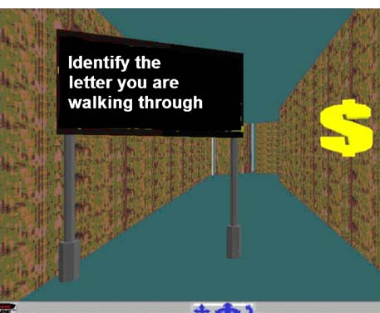
\includegraphics[width=90mm]{images/litreview/dsim1.png}
\caption{Image of dyslexia simulation}
\label{autisim1}
\end{figure}

\begin{figure}[H]
\centering
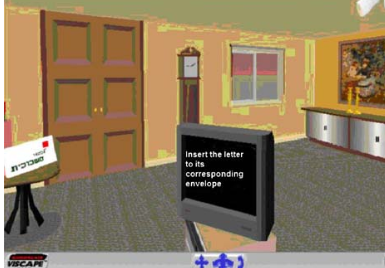
\includegraphics[width=90mm]{images/litreview/dsim2.png}
\caption{Image of dyslexia simulation}
\label{autisim1}
\end{figure}

Results of the study revealed a significant improvement of understanding and awareness in the experimental group whom played the VR simulation.

\begin{figure}[H]
\centering
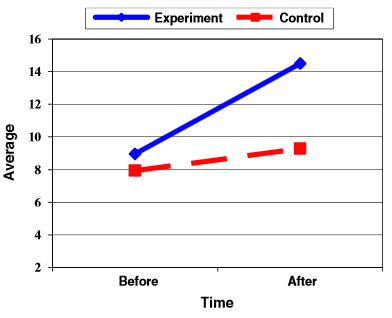
\includegraphics[width=90mm]{images/litreview/dsimresults.png}
\caption{Results of dyslexia simulation}
\label{autisim1}
\end{figure}

Physical disability simulations have been thought to hold disadvantages, potentially lead to pity and misconceptions \cite{dd}, for example the user might take a simulation literally that the experience is exactly what it is like to be all people with, dyslexia for example, rather than a potential representation and experience and understanding that every person is different and will be affected by symptoms in a different way.

A computer simulation may hold an advantage over physical simulations by being possible to depict developed cognitive advantages aspects such as heightened hearing (in the case of visually impaired). In addition computer simulations could highlight thinking differences by visualising the in-game character's thoughts and feelings when approached by various obstacles and these could be used to reduce pity or misconceptions.

In regards to the overall success of simulations, little research has be found to conclude the success or failure of using simulations as a method to raise awareness and understanding apart from \cite{dyslexicsimpar} which also specified "no studies have been made to date, of efforts to increase awareness of the cognitive aspects of the child with learning disability".

\subsection{Autism simulation and tools}

In February 2013 a playable 3D virtual environment depicting sensory difficulties in autism was released. The simulation involved the user navigating a school playground which contained other children whom all looked identical(to represent difficulties with facial recognition). If the user gets too close to the children, visual distortions and high-pitched sounds/screams are played. 

\begin{figure}[H]
\centering
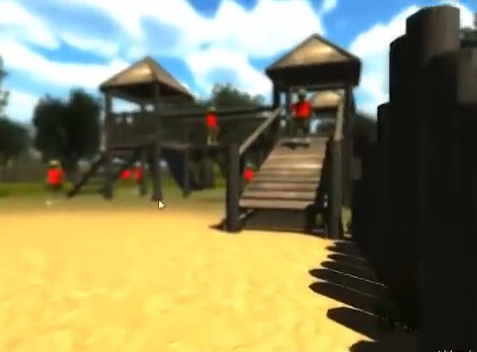
\includegraphics[width=90mm]{images/litreview/autisim1.png}
\caption{Image of playground with no sensory effects}
\label{autisim1}
\end{figure}

\begin{figure}[H]
\centering
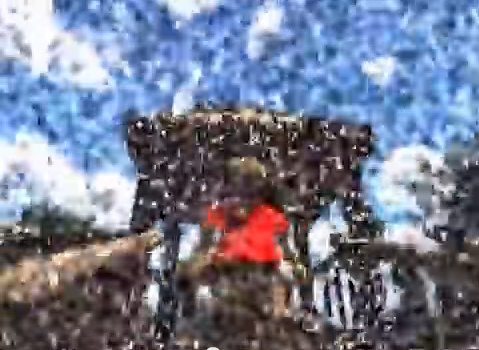
\includegraphics[width=90mm]{images/litreview/autisim2.png}
\caption{Image of playground with sensory effect distortions}
\label{autisim2}
\end{figure}


The simulation from the public was well received and regarded as a good step in increasing awareness and understanding of autism. From those with autism the feedback was mixed with some commenting the portrayal was not an accurate representation of their difficulties whilst for others it was, highlighting the breath of experiences these individuals have and the challenge of the task at hand.

In addition to a playable simulation some autistic individuals have created short videos to demonstrate the impact of sensory problems on their day to day lives and these have been very well received(Gary G. Porter). 
\begin{enumerate}
\item Video simulation of a sensory overload created by a group aiming to use media to help others understand autism: http://www.interactingwithautism.com/section/understanding/sensory/1
\item Video simulation of sensory overload in a supermarket created by an individual with autism: https://www.youtube.com/watch?v=IcS2VUoe12M
\item Autism simulation of a variety of aspects: http://simdis.jisctechdis.ac.uk/Autism/repres.htm
\item Video of sensory overload whilst an individual is walking along a street: https://www.youtube.com/watch?v=plPNhooUUuc
\end{enumerate}

One great benefit of conveying difficulties visually is that it helps obviates to some extent the ever-present language barrier and helping to overcome difficulty for people with autism.  

\chapter{Participatory Design}
Autism as previously described comes with a vast array of difficulties, some of which may be too complex or time consuming to convey(such as social difficulties). It was consequently important to select the most salient aspects of Autism and the participatory design was conducted to facilitate these choices and the design of the prototype. 

\section{LAER Lab}
An initial consultation was held with Learning and Adaptive Environments Research(LAER) Lab which aims to "bring together academics and students interested in technologies designed or applied with the goal of furthering education". In attendance were several members(I have little idea of who these were or how to describe them...you, Alyssa...) as well as two other students whom were also creating software projects related autism. An overview of the simulator was given in addition to goals and suggestions(see appendix for notes on what was given). Children are exposed to a plethora of different environment on a day to day basis(school, work, parks, etc), however, the most common location for a child is the home and thus by understanding the pitfalls and hazards around the house, knowledge should be transferable to other environments or domains. 

The consensus of the group was to restrict the simulator fist and foremost to conveying sensory differences in autism and to focus on the 3D home environment.

// think I still may have the actual document I took in all scribbled on. Or emails/feedback which may give indication of what happened.

\section{Interviews}
Interviews were conducted with five people and varied from teachers as well as adults with autism. Participants were recruited using the LAER labs participant network as well as a attendees to an Autism group.

\begin{enumerate}
\item Candidate one: teacher of a school for autistic children
\item Candidate two: special needs teacher of a school with varying disabilities.
\item Candidate three: parent of a teenager with Aspergers syndrome and ADD. Described themselves as neurodiverse having severe sensory difficulties but fewer social ones.
\item Candidate four: parent of a child with Aspergers syndrome and is themselves neurodiverse. Candidate describes having high sensory issues and fewer social ones.
\item Candidate five: person with high-functioning autism whom has higher social difficulties and fewer sensory.
\end{enumerate}


\subsection{Methods}
Ethical and consent forms were completed and participants all allowed for their interviews to be voice recorded. Interviews with teachers were conducted in the location of the schools. Interviews with candidates three and four were conducted at my own home and interviews with candidate five was conducted at their home. Candidates were in addition shown mock up images of sensory overloads(see figures \ref{sensorymockup1}, \ref{sensorymockup2}, \ref{sensorymockup3}) and asked for their feedback. 

Some interview questions were scripted however the interview topics varied as directed by the interviewees and dependant on the person's experiences i.e a teacher would be asked different questions to someone with autism. As interviews progressed there were improvements on questions asked. Some interview scripts have been included in the appendix however as they were auditorily recorded and some over an hour, not all information could be transcribed. Questions differed depending on the group: teachers were asked more specific questions in relation to their work and their feeling towards to the simulator concept. Adults with autism were asked more personal questions in relation to their own difficulties. 

\textbf{Summary of interview topics for Candidates 3-5}
\begin{enumerate}
\item Opinions and suggestions on the proposed project.
\item Most prominent difficulties faced on a day to day basis(as a parent or individual with autism).
\item In your opinion what is the difficulty that Neurotypical people find the most difficult to grasp about AS children.
\item Obstacles faced around the home environment
\item What would you regard as a successful day.
\item Explanation of sensory or meltdown experiences or triggers.
\item Problems in communicating difficulties.
\item Experiences in contending with mainstream schools.
\end{enumerate}

\textbf{Summary of interview topics for Candidates 1-2}
\begin{enumerate}
\item As you have years of experience with AS children, would you find it helpful if a simulator highlighting sensory difficulties, meltdowns ambiguous instructions was created?
\item In your opinion which topic should be highlighted as the most important within the simulator? 
\item If you had a trainee, what important information would they need to know and what aspects are the hardest to explain.
\end{enumerate}

Finally, all candidates were shown the following mock-up images of sensory overloads and asked for their feedback. 

\begin{figure}[H]
\centering
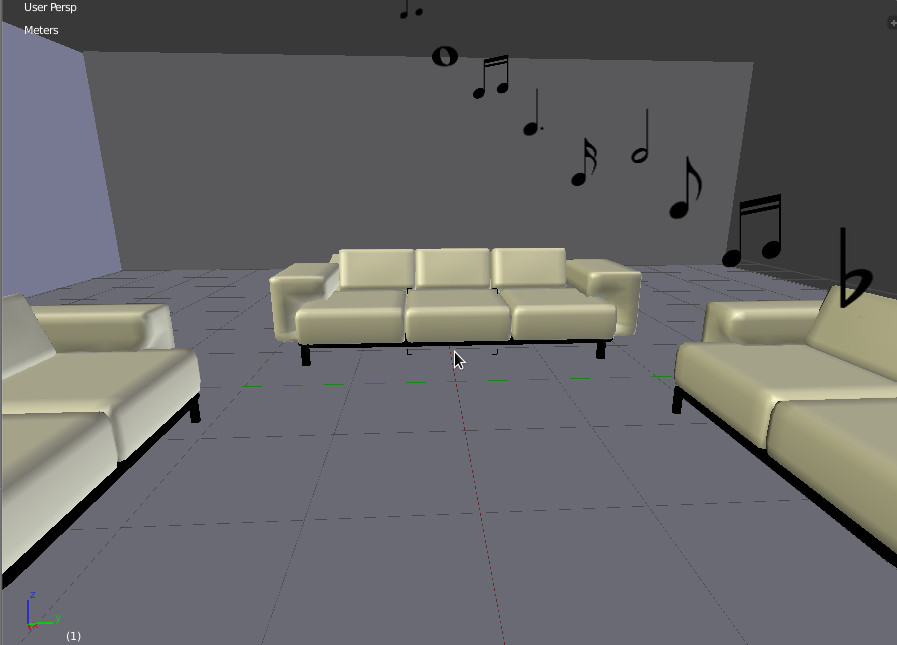
\includegraphics[width=90mm]{images/design/GD_basic.jpg}
\caption{Room with one object generating sound}
\label{sensorymockup1}
\end{figure}

\begin{figure}[H]
\centering
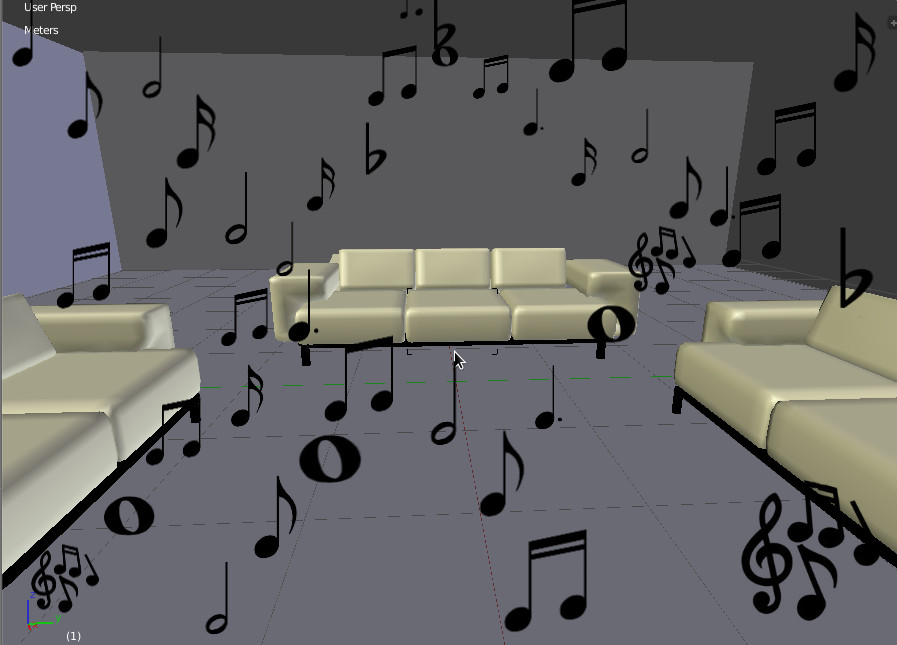
\includegraphics[width=90mm]{images/design/GD_moresound.jpg}
\caption{Effects of multiple objects creating sound}
\label{sensorymockup2}
\end{figure}

\begin{figure}[H]
\centering
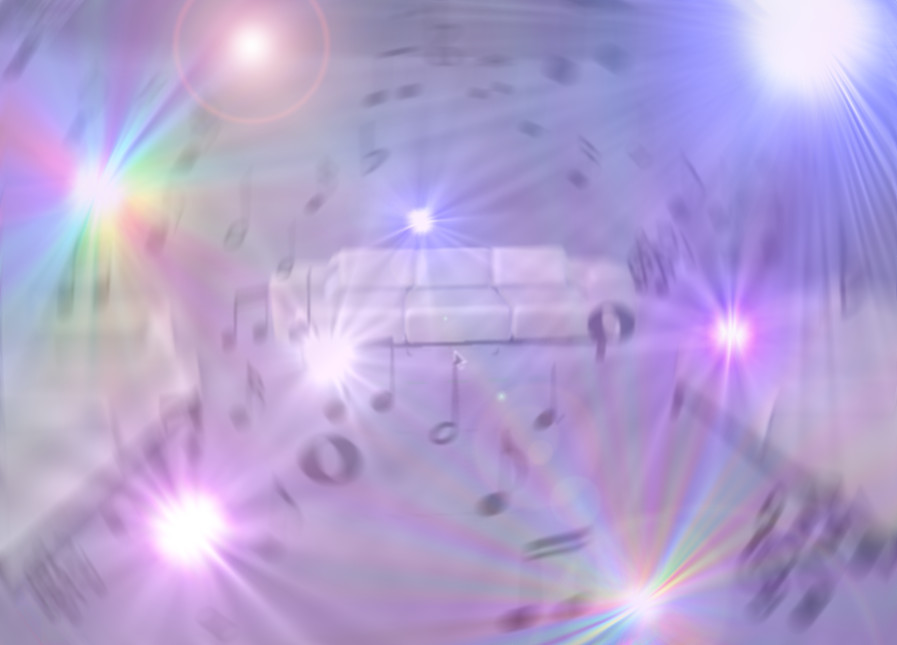
\includegraphics[width=90mm]{images/design/GD_overload.jpg}
\caption{Sensory overload. Lights have become brighter and environment is harder to see. Gaussian filter applied}
\label{sensorymockup3}
\end{figure}

\section{Results}
Interviews were an invaluable contribution to the project that gave insight and feedback into the Autism world currently not found from literature. As interviews were guided by the interviewee, some interesting and finding were observed. In addition, obtaining information from a teacher with large amount of experience in the domain revealed problems when new trainee teachers arrived and how they interacted with children with autism in class.  

Sensory difficulties was particularly prominent for two interviews "I was just so traumatised by the time I got to school with all these different noises, smells in the car and overload of sensory information. I'd just sit in silence and I couldn’t explain to anyone around me what was going on. When I finally arrived home, it just all came out as anger, rage even and my parents never knew why."[C3]. "The noises in the playground were just too much. So i'd sit by the edge of the playground and watch cars go past because those at least were predictable. I used to do this with slinkys on the stairs as well. The sound was beautiful."[C3]. [C4] also specified that for them to replenish energy a quiet environment was required and that "special interests" could be "literally used to replenish energy levels". [C4] in addition specified that as a child they would take coins around with them everywhere they went so they can spin them and use this to alleviate some of the turbulant sensory experiences "I used to do this in school and teachers didn't like that I wasn't paying attention to them. They didn't know that playing with them actually helped me to focus on what they were saying".

[C3] specified they were unable to communicate difficulties until much older however this is contrasted with another interview that felt "I'm pretty good at verbalising my problems, I've always been quite good at doing so although people don't always understand" [C5]. Although the prevalent theme of wanting more understanding was apparent, it was interesting to see the differences in obstacles faced and highlights the need for the simulator to be flexible. 

Changes in routine and structure were also highlighted a predominant cause of stress and anxiety as "A good day would be a structured day with no unpredictable events or changes in routine. Changes in routine can really make me anxious. And when I don't wake up with anxiety, sometimes anxiety can last for days. Also, if the weather is nice, that can help a good day" [C5]

The hardest difficulties highlighted by both teachers was "Language, communication and information processing delay. "A lot of staff have verbal diarrhoea and we have to keep reminding them to give black and white information or time to answer questions. Also the delayed processing of information where staff keep repeatedly asking questions without giving them time to think."[C2] and such events were said to sometimes lead to a meltdown. [C2] also spoke of the difficulty with contrasting sensory needs in the classroom, if a child required visual simulation which manifested as turning the lights on and off it could cause sensory issues for another child whom is sensitive. 


\section{Conclusions: Goals and restrictions identified}

2 of the 3 people interviewed specified that found the images of the sensory overloads extremely uncomfortable to view(and quickly looked away), and that it was an accurate representation. This demonstrated that a sensory overload differs for each individual and indicates more should be consulted as 3 is a small sample. However, the projects core aim is to raise awareness of these problems rather than attempting to give an identical experience of having autism and thus the mock images will be used unless feedback in the formative evaluation indicates changes are required. 

From the interviews conducted, the choice of project was solidified as well as the difficulties chosen to convey:

\begin{enumerate}
\item Sensory atypicalities: selected as the primary difficulty to convey due to their prevalence and hidden nature which is less known to the public
\item Meltdowns: As these can be caused by sensory atypicalities and it is important to convey to the user the impact of difficulties, not just the difficulties themselves.
\item Special interests: A means in the game to 'soothe' the character and counteract meltdowns.
\item Information processing delays: commented as a big problem in the classroom.
\end{enumerate}

Due to the complexity of conveying social and communication problems it was decided not to include this in the first version despite its prevalence in autism life. Sensory processing problems were selected as as this was a prominent theme in interviews and listening to individuals speaking of the trauma, the inability to communicate and seek help was really heart-felt. Information processing was selected as teachers highlighted this as a main cause to meltdowns in the classroom. 


\chapter{Prototype Design}
The role of the user will be to play as a child with autism and experience the world through their eyes, obtaining valuable insight and understanding as to what it may feel like to have these difficulties reducing inference and guess-work from literature(probably better explained what I mean in the sound part of "Redesign").

The primary target audience selected are teachers however, it should be developed such that anyone with little knowledge on autism and computer game experience can play and learn. To further achieve this, accessibility is an important consideration and where possible it should be made freely available on-line, making autism training a fun and interactive possibility for all, regardless of budget.  

Finally, instead of creating an overall architecture for the prototype it was chosen to simply implement features and allow the system to evolve due to current limited experience with JMonkey; the architecture would be likely rapidly change as issues arise, voiding any plans or design. For the second iteration of the design; a more in-depth plan detailing components of the system should be created.

\section{Game play}

The user will move around and explores a realistic home environment and be able to interact with objects such as turning off lights, opening and closing doors. Their well-being will be monitored at all times by a $contentment$ gauge visible on screen. Certain actions will result in this reducing, i.e a sensory overload or getting dressed and other interactions such as engaging with a special interest will increase contentment. If contentment drops to zero the player experiences a meltdown and restarts. 

\subsection{Interface and Controls}

Contentment as in the top right of \ref{design_interface_actions} is represented as a "health bar". When the user aligns the cross hair with an object and presses the action button, an interface will pop up with the actions currently available. On the top left of \ref{design_interface_actions} is the tool tip which will change depending on what object the cross hair is hovered over, indicate if there are any actions available. 

\begin{figure}[H]
\centering
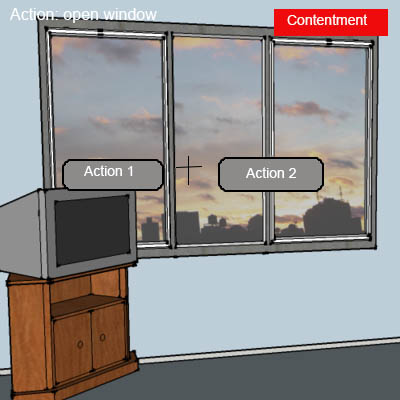
\includegraphics[scale=0.5]{images/design/interface_actions.jpg}
\caption{Mock up of contentment and action selection}
\label{design_interface_actions}
\end{figure}

Controls will be standard game controls commonly found in games. This should minimise learning involved in playing the game,  for current and novice game player alike: 

\begin{enumerate}
\item Mouse or direction buttons will be used to control the camera
\item W: move forward
\item S: move backwards
\item A: move left
\item D: move right
\item Space bar: action button for interacting with objects
\end{enumerate}

\subsection{User tasks: Mission and Explore mode}
Two modes in the simulator will be created, "Explore mode" and "Mission mode". Explore mode offers the user an opportunity to navigate the environment whilst learning how to deal hazards such as sensory overloads and meltdowns with less penalty than in the Mission mode. Explanations, hints and suggestions will be offered as the user has difficulty, for example after the first meltdown an explanation will occur explaining what has happened and that this occurs when contentment reaches zero. On the second meltdown occurrence a hint will be offered as a means to potentially avoid these in the future. In addition, this highlights interview-obtained information that children with high-functioning autism were unable to pinpoint what was causing them to meltdown until they were older and able to verbalise; they had to learn how to avoid situation through experience. 

Mission mode is a game mode that requires the user to complete specific tasks, apply and test their acquired knowledge and understanding from the explore mode whilst circumventing obstacles, in essence, this is the game or story mode of the program. Meta-cognition can be defined as "Knowledge about knowledge" and holds two key elements: Knowledge about knowledge, knowledge regulation which entails formulating plans as to fill knowledge gaps. By implementing the two different game-modes, an environment to learn and then later test it should aid meta-cognitive knowledge development in respect to autism. Users could acquire their own skills and strategies in dealing with these situations, and if some of their conclusions to dealing with these strategies are similar to someone with autism, it will aid understanding as to why some of the autism coping strategies are used.  

For the prototype version of the game, the Mission mode will entail two tasks: To get dressed and then proceed to obtaining a drink from the kitchen and hazards in the kitchen will include lights and a washing machine which will be placed next to the sink. For the first complete version a more in depth storyboard will be created with the aid of feedback from people whom have autism. 

\section{Simulator features}

\subsection{Description boxes}
Users will be able to click on certain objects and obtain information in the form of pop up boxes that may be of interest, hazardous or cause problems for someone with autism. I.e explaining that information on TV may be taken literally and a child may thus expect a toy to react in the same way as advertised or may not be able to identify that what is seen on TV is not real or explaining that clothes can literally feel like sandpaper. This information will be taken from literature and suggestions from people with Autism. 

\subsection{Sensory overloads}
Three sensory-types will be implemented; sound, light and tactile. The proximity and amount of objects around the player will firstly affect the sensory health(which is not visible to the user). When this falls below a specified threshold the first level of a sensory overload occurs and the impact of surrounding objects become more prominent, lights becoming brighter even if they were not initially interfering and causing the sensory overload and the contentment will slowly start to reduce. If the player does not move away, the second level is reached and the contentment bar reduction is rapid; visual effects worsen as the environment becomes more troublesome to navigate; representing a full sensory overload.

Following mock-ups and the positive response, two versions of a sensory overload were implemented and recorded before being sent via email to adults with autism to acquire feedback. The first was not well received or understood, however the second which was much closer to the previous mock images in \ref{sensorymockup3} had a strong positive response.  

One of the effects of sensory overloads was for lights to get brighter which can be easily conveyed in JMonkey using "Bloom" filters. A Guassian filter is suggested to make the overall environment harder to navigate and to mirror dizziness described when experiencing a full sensory overload. 

Finally, the sensory system will effect and be affected by the contentment bar. Interviews showed that if someone with autism is feeling particularly drained from their day or awakens feeling particularly anxious their tolerance to surroundings is lower and hence when contentment is lower, a sensory overload is more likely to occur. If the user is around no interferences or people, contentment will slowly increase. 

\subsection{Meltdowns}
Meltdowns occur when someone with Autism becomes stressed or overwhelmed. This will be represented as 'Contentment' drawing comparison to a "health bar", commonly seen in games. There have been multiple suggestions to convey this:

\begin{itemize}
\item During a meltdown, make the character harder to control. When pushing "right" the character instead moves left and vice versa.
\item Make the screen blackout and reopen with items in the house destroyed.
\end{itemize}

The first option was selected and moulded for the prototype. As contentment gets closer to zero, the camera will shake, giving the player a few seconds to attempt to prevent the meltdown. The closer contentment gets to zero the more the camera will shake. When contentment reaches zero, a meltdown will occur and the player will restart in the bedroom. 

\subsection{Special interests}
'Special interests' were chosen as a way to alleviate some of the difficulties within the environment and replenish contentment. When engaging with a special interest, troublesome sounds will be reduced and if experiencing a sensory overload or meltdown the effects will subsidise. The special interest selected will be a Dinosaur toy which the user can interact with.

\subsection{Information processing delay}
Information processing delay was highlighted in interviews by a teacher as one of the main causes of meltdowns in school. When the user clicks on an object to interact or is expected to give a response, actions will be made harder to select by rotation around the screen. If the character has lower contentment the selections will move even quicker which should result in a greater delay from the player as it becomes more difficult to click them. Such delays could later affect responses from other characters in the game; if the user does not respond quick enough an in-game character such as the parent will prompt the user to hurry up, causing contentment to further drop and the actions to rotate quicker. It was highlighted in the lit review that if someone with autism is interrupted during information processing, they have to start over again but it becomes harder due to stress and anxiety. 

\section{Tool selection}
A game engine was selected to allow focus to be directed onto higher level concepts of the simulator. Suitable game engine candidates as well as modelling tools were identified by looking at those highly rated on gamedev.net (extensive online resource for game developers), whilst taking some previous knowledge into account. After narrowing choices to a few, the advantages and disadvantages were weight up and a choice was finally made. 

\subsection{Game engines}

\begin{table}[H]
    \begin{tabular}{| p{2cm} | p{4cm} | p{6cm} | p{5cm}| }
    \hline
    Engine & Description & Advantages & Disadvantages \\ \hline
    Unity & Unity is one of the most popular game engines available with good support for models. Unfortunately the licence costs 1500 and the free version comes with limitations. & \begin{minipage}{6cm}
    \vskip 4pt
    \begin{enumerate}
   \item Popular game engine to use with a large support base and model repository. 
   \item Quick development with scripting, games with impressive graphics can be made quickly. 
   \item Phone app support.
   \end{enumerate}
   \vskip 4pt
 \end{minipage}   & 
 \begin{minipage}{5cm}
    \vskip 4pt
    \begin{enumerate}
   \item Interface heavy 
   \item Limited to scripting rather than having control of whole game architecture
   \item Costs 
   \item Good computer required to run it efficiently.
   \end{enumerate}
   \vskip 4pt
 \end{minipage}
	\\ \hline
	JMonkey & JMonkey is a java 3d game engine that has been in development around for a few years. It has an extremely active and helpful community, allows complete customisation and holds little limitation being open source.  &
	 \begin{minipage}{6cm}
    \vskip 4pt
    \begin{enumerate}
   \item Provides development environment in addition to a scene graph.
   \item Active community where you often get responses from developers themselves.
   \item Java is quick to develop in enabling focus on higher level features.
   \item Support for online use and phone apps aiding goals of accessibility.  
   \end{enumerate}
   \vskip 4pt
 \end{minipage}  
 & 
 	 \begin{minipage}{5cm}
    \vskip 4pt
    \begin{enumerate}
   \item Java is not seen as the preferred language for graphics or games.
   \end{enumerate}
   \vskip 4pt
 \end{minipage}  \\ \hline
 Panda3D & Originally created by Disney, Panda3D is an engine which can be used via python or C++ although support is mostly for python. & 	 \begin{minipage}{6cm}
    \vskip 4pt
    \begin{enumerate}
   \item Quick to develop for with a choice in language.
   \item Good community with lots of tools.
   \end{enumerate}
   \vskip 4pt
 \end{minipage} &  \begin{minipage}{5cm}
    \vskip 4pt
    \begin{enumerate}
   \item No phone app and limited online support. 
   \item Lack of documentation. 
   \end{enumerate}
   \vskip 4pt
 \end{minipage}
    \\ \hline
    Ogre3D & Ogre3d is primarily a graphics rendering engine and but it does have additional plugins such as 'physics' or drawing interfaces &  \begin{minipage}{6cm}
    \vskip 4pt
    \begin{enumerate}
   \item Lots of modules and plugins
   \item Active support community
   \item Open-source
   \end{enumerate}
   \vskip 4pt
 \end{minipage}
 &  \begin{minipage}{5cm}
    \vskip 4pt
    \begin{enumerate}
   \item Longer development process
   \item Lack of tools such as a scene graph. 
   \item No online support
   \end{enumerate}
   \vskip 4pt
 \end{minipage}
    \end{tabular}
\end{table}

JMonkey was chosen for its active community, development environment being open source and programmed in Java and open-source. Although Java is not seen as the programming language of choice for graphics it enables quicker development than C++ counterparts. Unity allows speedy quick development with great results but the pro version would be required for some features which is very expensive. As JMonkey is in Java put online with ease, increasing accessibility. Finally there were no foreseen limitations with using JMonkey a part from concerns about performance which may become an issue at a later date.

\subsection{Modelling tools}
For modelling there several options available:
\begin{itemize}
\item Maya
\item 3DSMax
\item Blender
\item Sketchup
\end{itemize}

Both Maya and 3DSMax are considered the industries leaders in modelling, animations and effect creation. However, they are both extremely expensive, costing over £3000. Sketchup is a google product, giving a wealth of models however its ease of use for beginners comes at a cost; it is not well supported for games although sketch-up models can be ported to other modelling software and edited to be more suited. Blender is an open source 3D modelling program with quick updates and the choice of tool for many game developers although has been thought to have a steeper learning curve than 3DSMax.

Blender was selected as the primary modelling tool for the creation of game assets, as there is little lost in using it in-spite of being free. It is widely used by game developers and professionals and is the tool JMonkey is most built to accommodate.

\chapter{Prototype}
The prototype was created as previously described and was followed by two formative evaluations. One with LAER Lab and the second in the form of an on-line questionnaire after participants watched a video demo. 

\section{Game play}

\subsection*{House environment overview}
The environment consisted of two bedrooms(one empty), a kitchen and a living-room, an overview of which can be seen in \ref{old_house}. It was kept open with no doors and thus no loading required between rooms. The house architecture was designed in sketchup and imported into Blender to be tidied and imported into JMonkey. Some models (such as furniture and the character) were taken from on-line resources such as blendswap.com.  

\begin{figure}[H]
\centering
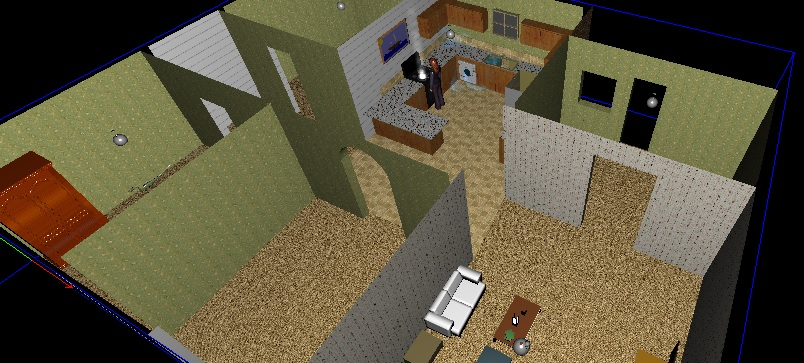
\includegraphics[width=90mm]{images/prototype/old_fullhouse.jpg}
\caption{Overview of the house used in the prototype}
\label{old_house}
\end{figure}

The living room in \ref{prototype_livingroom} contains three interact-able objects, a TV, lamp on the table as well as a ceiling light, the latter two which affect the sensory system and if not turned off or the user is too close can result in an overload. 

\begin{figure}[H]
\centering
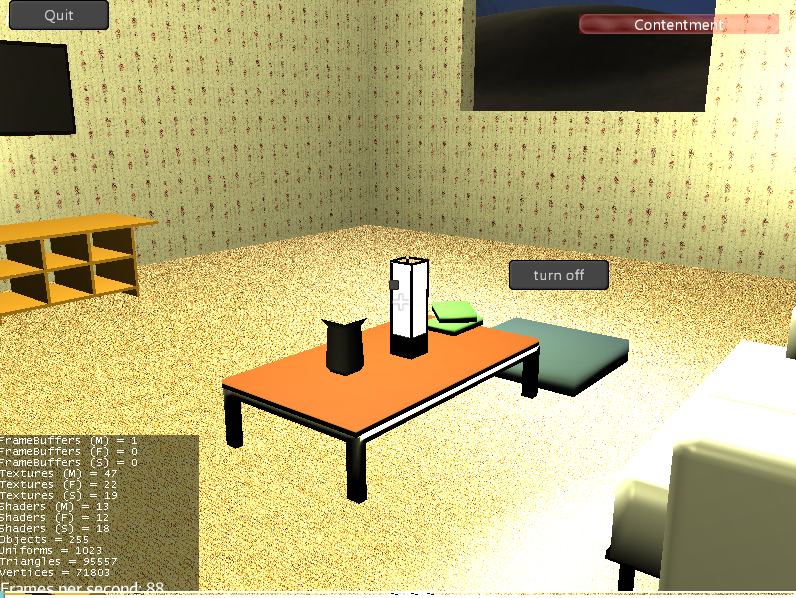
\includegraphics[width=100mm]{images/prototype/livingroom.png}
\caption{Livingroom}
\label{prototype_livingroom}
\end{figure}

The players bedroom consisted of a bed, wardrobe, ceiling light and "special interest"; a dinosaur which the user could interact with.

\begin{figure}[H]
\centering
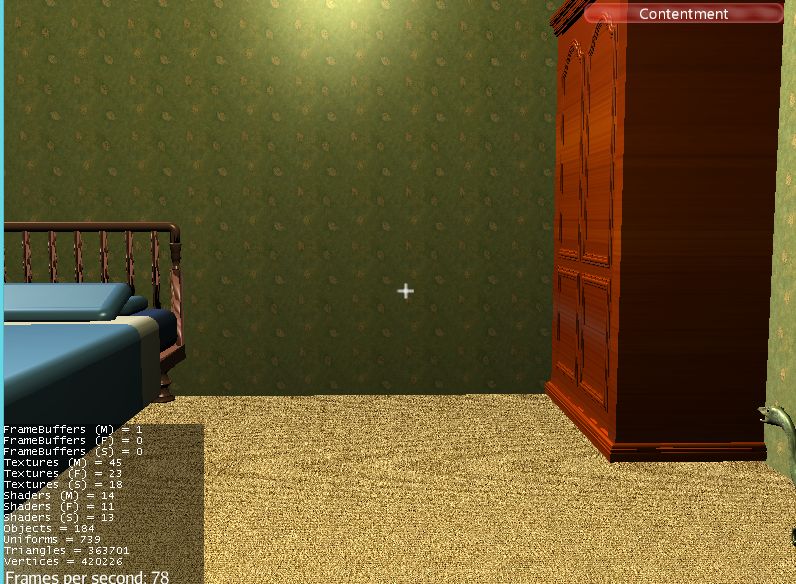
\includegraphics[width=100mm]{images/prototype/bedroom.png}
\caption{Bedroom}
\label{prototype_bedroom}
\end{figure}

The kitchen contained the parent of the game, a washing machine and ceiling light all of which were interactable. The washing machine could be turned on and off which effects the visual effects of sounds. Music notes were primarily to be used in the design, however the wanted effects could not quite be obtained and so sound waves were used instead.  

\begin{figure}[H]
\centering
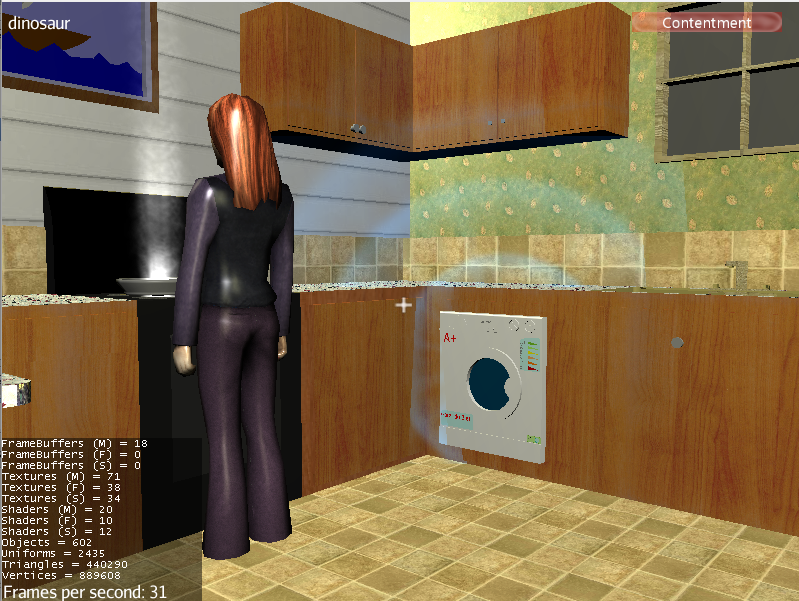
\includegraphics[width=100mm]{images/prototype/kitchen_washingm.png}
\caption{Kitchen: Visual effects from the washing machine can be seen}
\label{prototype_kitchenwash}
\end{figure}

Finally, as the game was open the user could venture outside(useful for running off if a sensory overload was occurring)

\begin{figure}[H]
\centering
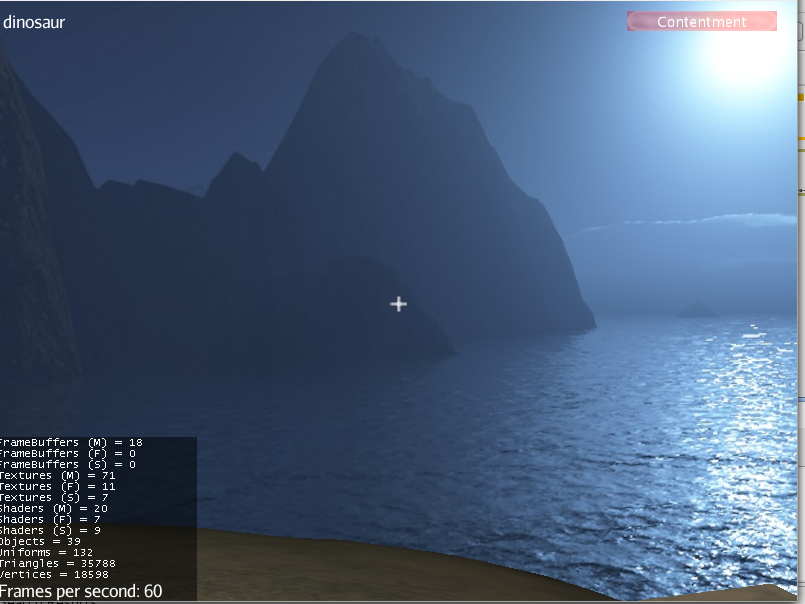
\includegraphics[width=100mm]{images/prototype/outside.png}
\caption{The peaceful outdoors!}
\label{prototype_kitchen1}
\end{figure}

\subsection*{Interactions}

The user can interact with various objects in the scene; some would provide information in the form of description boxes whereas others directly affected game play such as lights and special interests. When available actions appear for selection, the camera is disabled enabling the user to select them with their mouse as can be seen in \ref{prototype_dino}.

\begin{figure}[H]
\centering
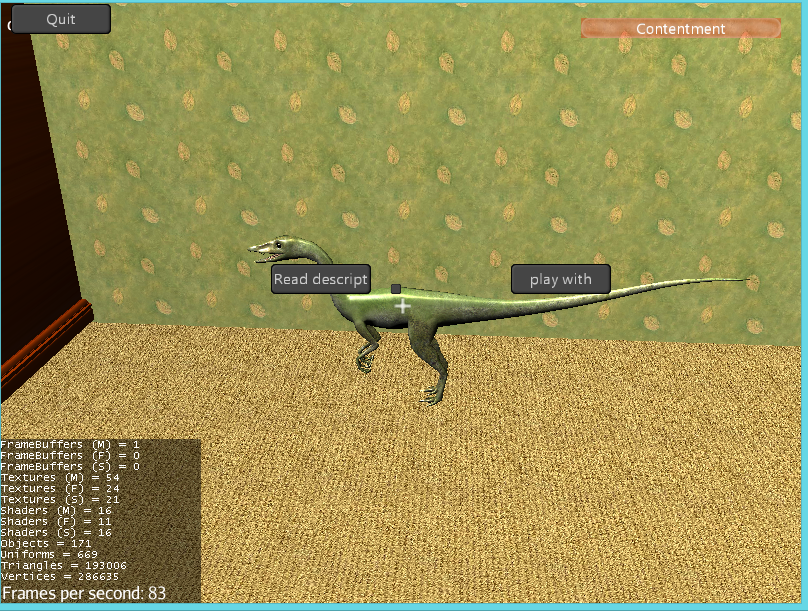
\includegraphics[width=100mm]{images/prototype/si.png}
\caption{Interacting with a special interest. Two actions available for selection can be views}
\label{prototype_dino}
\end{figure}

When the user interacts with the dinosaur(\ref{prototype_dino}), contentment increases although there was little visual indication of doing this(apart from the contentment visually increasing) and if the player was far away from the object, playing would stop. If a sensory overload was occurring and the player moved to the dinosaur quick enough they could prevent a meltdown by increasing contentment although interacting with the object would not specifically stop sensory overloads and should be implemented at a later date. 

\begin{figure}[H]
\centering
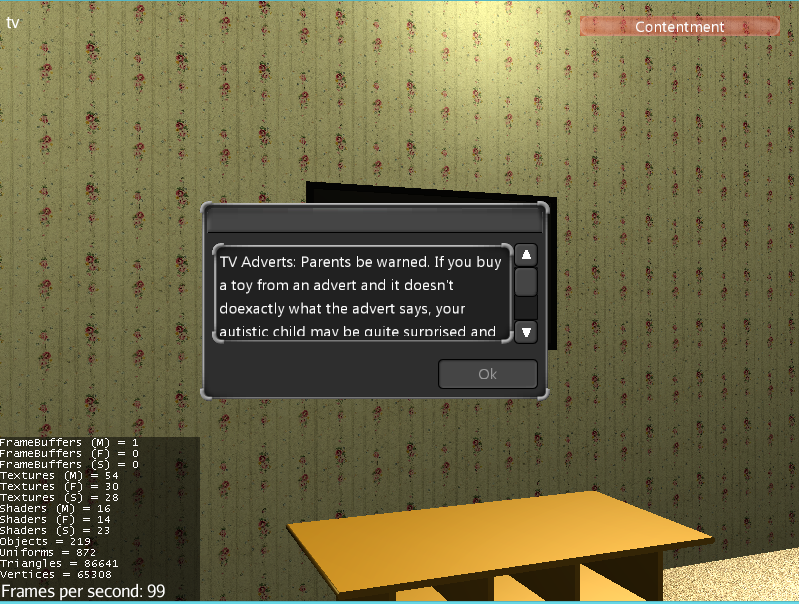
\includegraphics[width=100mm]{images/prototype/tvdescription.png}
\caption{TV description box pop-up, giving warnings of that a child may literally interpret what they see on TV }
\label{prototype_tvdesc}
\end{figure}

Only a few descriptions in the prototype were implemented. Wardrobe, frying pan, TV, dinosaur and one of the issues that arose came during sensory overloads. If one was occurring whilst reading a description the user either had to close it quickly and move away or continue to read and risk a meltdown; which if this occurs the game will reset and the user won't be able to view the description information. This is not ideal behaviour; preventing useful or important information being read.

\subsection*{Sensory overloads and meltdowns}

Sensory overloads occur when being too close to too many hazardous objects and it was was broken down into two stages, the first of which results in lights and the environment becoming brighter as can be seen in \ref{prototype_so1s1} and \ref{prototype_so2s1}. 

\begin{figure}[H]
\centering
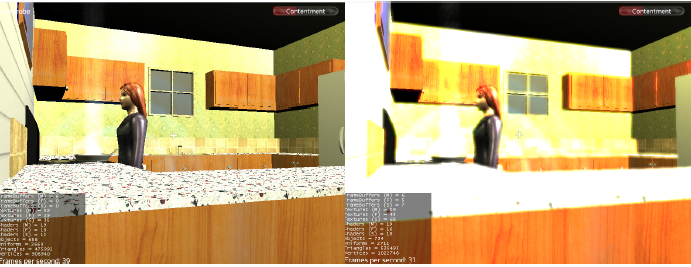
\includegraphics[width=100mm]{images/prototype/old_sensoryeffects.png}
\caption{Sensory overload effects at stage 1: The image on the left demonstrates a view with no effects. The image on the right is the result of the Bloom filter being applied resulting in lights and the environment becoming brighter}
\label{prototype_so1s1}
\end{figure}

\begin{figure}[H]
\centering
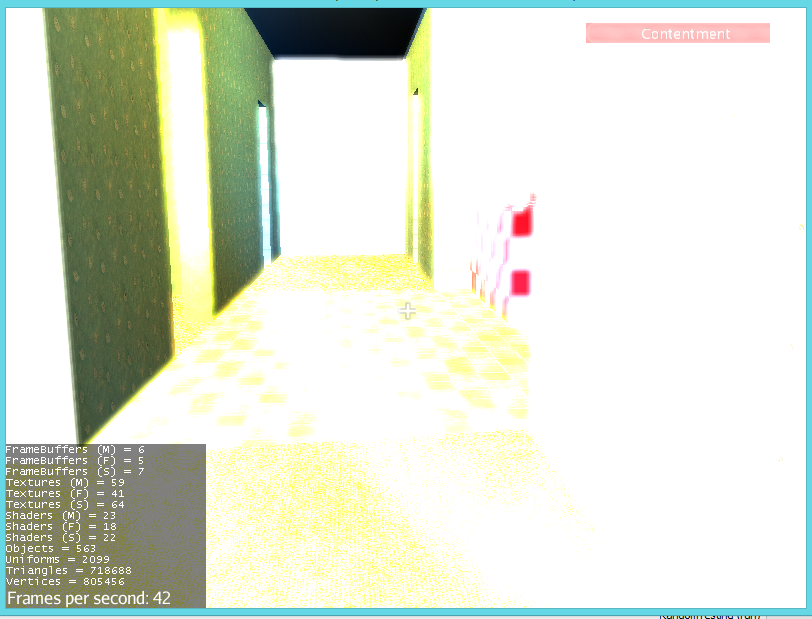
\includegraphics[width=100mm]{images/prototype/hallway_so1.png}
\caption{Sensory overload effects at stage 1: hallway extremely bright as there's lots of lighting causing issues}
\label{prototype_so2s1}
\end{figure}

If the user does not deal with this quickly enough by turning off the source of disturbance or moving away the second stage is entered which can be seen in \ref{prototype_so1s2} and \ref{prototype_so2s2}. 

\begin{figure}[H]
\centering
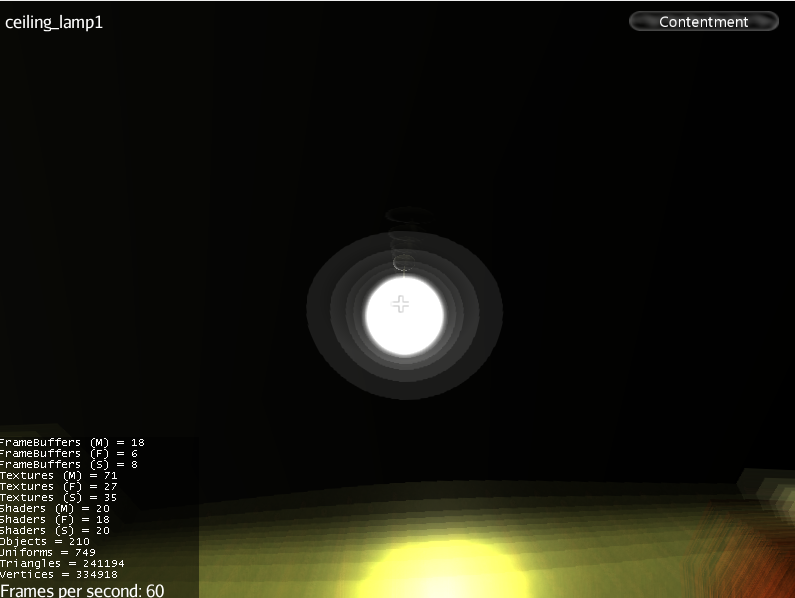
\includegraphics[width=100mm]{images/prototype/bedroom_lightsensory.png}
\caption{Sensory overload effects at stage 2: Light is much brighter and the Gaussian blur filter is applied}
\label{prototype_so1s2}
\end{figure}

\begin{figure}[H]
\centering
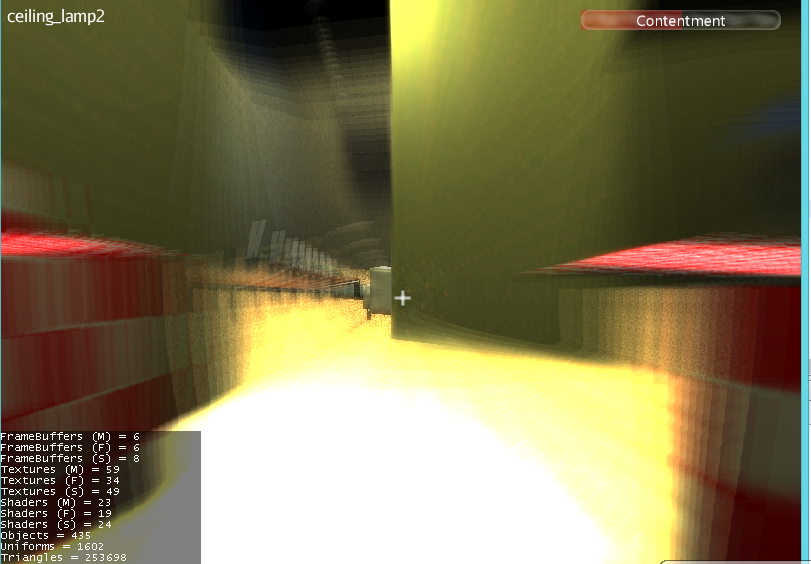
\includegraphics[width=100mm]{images/prototype/so_kitchen.png}
\caption{Sensory overload effects at stage 2: Gaussian blur filter is applied and full sensory overload is occurring}
\label{prototype_so2s2}
\end{figure}

Translating the information from interviews and readings to implementation had proved challenging because of the amount of differing information. The specific triggers do require work and adjustment, for example having only certain types lighting causing problems as currently all of them are. In addition, certain lights should only cause sensory overloads when the user is looking directly into them. Sound is currently represented by visual sound waves emitting from objects and these need to be made bigger and more dense as to cause more visual distortions.

\subsection*{Game modes}
When the simulator first starts the user can select either Explore or Mission mode with a few other options such as "About" and "Help". These cannot be switched during play and the simulator needs to be restarted to change modes. 

In mission mode, two tasks were given: to get a drink and to get dressed. When the user gets dressed, contentment drops due to tactile sensory problems; on completion(assuming the character does not have a meltdown) the next mission is selected. 

Next to the sink as in \ref{prototype_kitchenwash} is the washing machine which combined with the lighting quickly creates a sensory overload. As a representation of "Getting a drink" an action indicator(similar to a health car) is used(see \ref{prototype_actionindicator}) and when displayed the user cannot move. It slowly reduced over time and upon completion the user can move again. Thus, they are fixed at the sink until the action of getting a drink is complete, having a few seconds to run or move away before a meltdown occurs. If the contentment is too low before the task is attempted a meltdown will occur during it and in either case, the player restarts in the bedroom to attempt again. 

\begin{figure}[H]
\centering
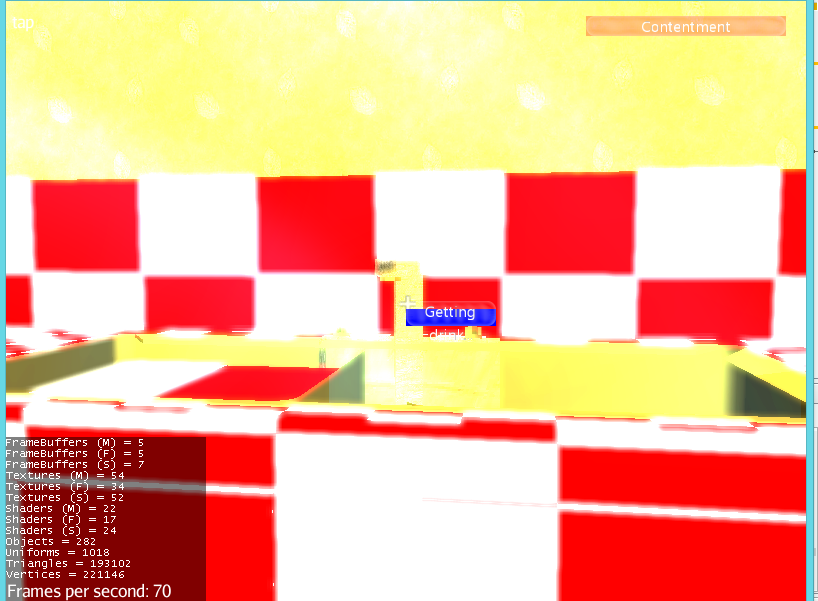
\includegraphics[width=100mm]{images/prototype/actionindicator.png}
\caption{Blue action indicator: (Texture is broken in the prototype when I tried to take this image which is why things are appearing red and white, not hard to fix but no need atm)}
\label{prototype_actionindicator}
\end{figure}

\section{Implementation architecture}
At the time the prototype was developed, a new GUI package became available for JMonkey although it is still in beta with little documentation. 

I'm not entire sure what is needed in this part and to what level of detail???

- scenes
- object states
- player class
- gui
- action manager
- class diagrams

\subsection{Missions}
"Missions" are represented as java classes and as such can be individually dropped into the system and loaded. These classes can define custom actions on objects which may only be applicable when the task is active, e.g, get a drink, get dressed, ask Mum for help. Task classes set the conditions for completion such as player is holding a drink, is dressed, spoke to mum and on completion the next task is selected and displayed to the user. One of the benefits of this comes with testing as specific tasks can be selected and it doesn't require going through a series of events to trigger the tasks that need to be checked or needing to comment out large portions of code.

\section{Overcoming challenges}

// hmm, maybe move this to a discussion section? Pretty sure there's more I can yap on about here. 

At the start of the project significant amounts of time were spent trying to import rather than create models. It was a tedious task because small changes to the models required the whole house scene to be remade in JMonkey or
time had to be spent on editing models better work with JMonkeys import system. It also became evident from using Blender that it has a very steep learning curve and is a tool which can take some considerable time to master.
However, in the last two months of the game development process, these obstacles have been largely overcome. Experience acquired, coupled with updates in February to the JMonkey import system, made it easier and less
time consuming to acquire, create, change and import models. The whole scene was no longer required to be rebuilt allowing time to be better spent. Moreover, the update allowed direct use of google sketchup, a 3D modelling
tool which is easier and quicker to use than Blender (although it produces less quality assets) and offers a wealth of free models in the online repository, most of which are home components such as furniture.

Overall, JMonkey has proven to be a good choice. No additional limitations have been found and development was quick once a solution was found to the model import pipeline. The modularity offered by Java allows
further extensions to be created with ease without needing to change a large portion of the program structure. Finally, being able to combine sketchup and Blender has been a great help and with practice, asset creation should
continue to speed up.

\chapter{Formative evaluation: Prototype}
The current version of the simulator has been evaluated in two settings. The first was the presentation of the simulator to LAERLab. The second was a questionnaire sent to some parents/family members of children with autism and adults with autism.

\subsection{Expert feedback: LAERLab}
The LAER group consists of students and academics with an interest in the field of accessible and educational technology design and 10 members provided comments and feedback.

A short video demo was presented and narrated showing exploration of the environment followed by one task being completed (obtain a drink from the kitchen). The demo included sensory overload effects, meltdown and information processing delay concepts. (**linux died on my laptop that I had used on the day and I'm pretty sure don't have this video!! Unless I sent it to other people via email. Should I just make another? )

\subsubsection{Results}

\begin{enumerate}
\item Lab members disliked the popup information boxes as they felt it interrupted the simulation. It was suggested information may be better put as a sidebar or bottom bar.
\item Made clear that the simulation information provided in the description boxes are just samples of things known to present problems to children with autism and do not represent all children with autism.
\item Idea put forward to allow the user to select the different issues relating to autism and then to test the consequences of this in the environment. 
\item Demo was a bit too quick, one of the problems being the camera is controlled by the mouse and the video was recorded on a laptop (so camera motion was not smooth). The general controls are quite sensitive.
\item Suggestions for tactile sensory when touching objects(create a slightly red blur around the edges as is common in games).
\end{enumerate}


\subsection{User feedback}
A video demo was briefly put on-line with verbal narration of what was happening in the simulator. No information on goals or target audience was given as users were asked whom they felt it would be useful for. The questionnaire which was completed by 1 family member of someone with autism, 3 parents of children with autism and 3 adults with autism. It contained both qualitative and quantitative questions. Some users chose not to respond using the questionnaire but gave comments. 

*** Reminder to self. Think I saved a massive amount of feedback on this where people didn't use the questionnaire; get from desktop.

\subsubsection{Results}

\begin{table}[H]
\caption{Questionnaire results. Participants responded giving an answer between 1 and 5. 5 being the highest rating}
\begin{tabular}{| p{9cm} | c c c c c |}
\hline
\textbf{Question} & 1 & 2 & 3 & 4 & 5 \\
\hline
How likely would you be to play the simulator? & 0 & 0 & 1 & 2 & 4 \\
\hline
How much do you think playing the simulator could help you understand the behaviour of a child with autism better? & 0 & 0 & 0 & 2 & 5 \\
\hline
How much did you like the visual effects? & 0 & 0 & 1 & 3 & 3 \\
\hline
How much did you like the graphics? & 0 & 0 & 2 & 2 & 3 \\ 
\hline
\end{tabular}
\end{table}

The qualitative questions asked were:
\begin{enumerate}
\item What is your experience with autism? (for example if you are a parent, professional, family member or someone with ASD yourself)
\item Who would you think the simulator would be useful for?
\item How accurate do feel the representation of a sensory overload is? Please include any additional comments.
\item Do you have any other scenarios, examples or information(that could go in description boxes for example) that could be offered that you think may be useful for others?
\end{enumerate}

Some of the responses to qualitative questions can be seen below, some participants chose not to give qualitative answers and only responded to quantitative questions:

*** appendix with brief summary and analysis?

What is your experience with autism? (for example if you are a parent, professional, family member or someone with ASD yourself)
\begin{table}[H]
    \begin{tabular}{| p{3cm} | p{12cm} |}
    \hline
     Participant & Comments \\ \hline
     1 & Parent of two ASD children. I also have ASD traits which may be aspergers. \\ \hline
     2 & I have a son now aged 15yrs diagnosed at Peterborough aged 3yrs 9 mnts by child development specialist and her team. Who gave enormous help in getting Tom into nursery and then school and regular assessments. We moved back to Ireland my home place when Tom was 6yrs and have had no help since(mistake). Tom has not been in school for more than 3 weeks since age 12yrs due to sensory issues and has recently started taking prozac for anxiety, which has helped enormously! Your simulator is a brilliant idea which will be a major asset to both parents educators struggling to understand a childs condition. There are so many scenes and scenarios that this can cover and it could be extended to outside the home to school and outside spaces! One example - I remember when Tom was about 5/6, we were at the park and it started raining so we headed home as we rounded the last corner Tom stopped and wanted to go back to start of corner! This was repeated 5 times and he was getting more and more annoyed starting to scream. He was insisting we go back again and it was pouring rain, in the end I said thats it and I ran down the road to the house and peered out and he eventually tottered down the road! But it took me ages to figure out what the problem was until I realized it was that every time we started to go round the corner a car came and the engine noise affected/disturbed his action/experience/sensation of something we take for granted and would not notice. A video simulation depicting such sensory agitators would make an enormous difference to carers and how they react to situations. Hope you found my reply helpful I have many examples such as how buttons on his school clothes caused meltdowns every-morning or how the simple task of changing a nappy was hell until we learned to talk the child through in stages. Best regards  \\ \hline
     3 &  I'm autistic  \\ \hline
    \end{tabular}
\end{table}

Who would you think the simulator would be useful for?
\begin{table}[H]
    \begin{tabular}{| p{3cm} | p{12cm} |}
    \hline
     Participant & Comments \\ \hline
     1 & Teachers, teaching assistants, health care professionals, families. \\ \hline
     2 & - \\ \hline
     3 & People who don't know much about autism - eg a teacher with an autistic student \\ \hline
    \end{tabular}
\end{table}

How accurate do you feel the representation of a sensory overloads are? Please include any additional comments.
\begin{table}[H]
    \begin{tabular}{| p{3cm} | p{12cm} |}
    \hline
     Participant & Comments \\ \hline
     1 & I have sensory difficulties so I felt uncomfortable when it became brighter plus the talking. That is me though and I have these sorts of experiences a lot. Not sure how it would feel for someone without sensory issues. \\ \hline
     2 & I think the reactions in the kitchen is good, maybe for other subtle agitators thought clouds could be used! Plus I think the simulator could be used in schools etc in educating young people, but I might prefer to maybe watch as a video if it were possible to have both formats!! \\ \hline
     3 & A lot more severe than how I experience it, but then I've got milder issues than many I know. But the only kids I know who'd go into a full meltdown that quickly from being near a washing machine would be low functioning (eg minimally verbal) so you may want to back it off a bit. (A fire alarm, on the other hand, would get that strong a reaction even from me.) I really like the effect of the swirling options. It's really unexpected, how well it captures what trying to speak when overloaded is like. I'd never have thought of that analogy, but it's perfect. \\ \hline
    \end{tabular}
\end{table}

Please let me know if you have any other general feedback on the simulator. E.g improvements, suggestions or what you would change.
\begin{table}[H]
    \begin{tabular}{| p{3cm} | p{12cm} |}
    \hline
     Participant & Comments \\ \hline
     1 & Felt more could be done with illustrating the pain of noise. Wasn't sure if the simulator did this; I was watching it rather than listening:( Hard for me to do both online. \\ \hline
     2 & - \\ \hline
     3 & Would it be possible to allow the user to chose between 1st and 3rd person mode? I find 1st person really hard to navigate in. \\ \hline
    \end{tabular}
\end{table}

Do you have any other scenarios, examples or information (that could go in the description boxes for example) that could be offered, that you think may be useful for others?

\begin{table}[H]
    \begin{tabular}{| p{3cm} | p{12cm} |}
    \hline
     Participant & Comments \\ \hline
     1 & Try to include some of the good parts of autism as well. For example, I really enjoy sparkly things. If you make him like sparkly things too, maybe you could highlight the sparkly things and make them look extra awesome to show that.  \\ \hline
     2 & - \\ \hline
     3 & I think if you could use the thought clouds as the avi walking around he/she can be expressing discomfort ie hearing unwanted noises etc my son used to be terrified of the vacuum cleaner! So many little things too! \\ \hline
    \end{tabular}
\end{table}


\section{Conclusions}

Following constructive feedback from these sources, the following amendments to the simulator have been selected:

Description boxes: the HUD can to be changed such that information on the environment does not affect game play. Descriptions could be implemented instead as 'thoughts' which would be displayed at the bottom of the screen and when looking at certain objects. An alternative would be to have a 'Task' which would simply enable no other game play apart from exploring and obtaining information on surroundings, whilst still retaining the pop-up boxes. Images could also be included to give better impact for example when explaining that clothe labels can feel like barbed wire to someone with autism an image of barbed wire and the information can be shown.

Meltdown system: contentment needs to simply reduce less when there are sensory problems around the environment although certain sound objects or lights may need to give more impact than others. I.e a fire alarm causing more problems than the sound of the tv. An internal action such as 'close eyes' might also be used. 

Game play: remove mouse for controlling the camera and allow simple arrow direction keys to be used. Also adjust the player movement so it closer resembles walking. Additionally implement an internal action 'run' to allow for faster movement although one suggestion would be for this to increase the chance of bumping into objects of falling over. 

Interface: User instructions for the start of the game need to be implemented as well as menu's and options for enabling or disabling certain sensory effects as viewers with autism commented they found it difficult to watch as it was causing them to have a sensory overload. 


\chapter{Redesign}
// this part isn't really done or changed apart from the "Sounds section". At the moment it has both implementation and design stuff.

Large parts of the system were rewritten and improved upon such as the GUI and sensory manager. The benefits resulted in simplification of use at the higher level (such as implementing storyboards) and a better representation of the causes of sensory overloads.

Selecting actions to interact with objects is now less intrusive. Prior a menu would pop up and prompt the user to make a selection with their mouse which will now only happen if there are multiple options. With the removal of description boxes, thoughts are now displayed at the bottom of the screen when to user is looking at a specific object.

Performance issues which were not previously too severe now required direct attention. The game requires a frame rate of 30fps(frame per second) or above in order to be fluent and played without lag. Scenes are required to have a maximum of 100k vertices(from models) with an average of 10-50k. Each pointlight(which is a light the user can turn on/off) used requires the scene to be rendered again and so the number of vertices double with each point light used. Thus, even when keeping within the limits, the amount of lights being used in the game was pushing it to well over a million and the frame frequently dropped below the desired threshold. This was occurring on a computer with a decent processor and graphics card, thus playing on a low-powered machine would not be a good experience.  

Having originally taken a large amount of models from other websites and using programs such as sketchup to aid quicker development, these were found to be inefficient at runtime. Efforts therefore were spent on re-learning the details of blender and what is required to make lightweight game models. 

Where previously the entire house modelled and then imported, the solution to the above problem was to split the house into individual rooms/scenes. When the user then clicks a door, the required scene is loaded very quickly. This approach allows for inclusion of more detailed models within each scene as each scene is only a small room. The problems to performance caused by point lights is then reduced as it is only rendering a single room again, not the entire house. 

Further benefits from compartmentalising the house into rooms arose for dealing with the model pipeline. It became much easier to create individual models and link them into the scene, so if the model needed to be edited it could be without requiring the pain of reimporting and fixing textures or materials. 

The result of the restructure meant the FPS improved tenfold, from an average of 30fps to 200-400fps. If any objects were found to be creating problems from being too detailed or not textures properly, they could be removed without impacting on the rest of the scene.

\section{Storyboards}
Following the prototype which had little story or goals, a more in-depth story and set of tasks were created. The user will play as an example "Day in the life of a child with autism". This will be split up into several "Missions"(tasks). The initial story was developed with consultation from two individuals; One was an adult with autism whom has a child with autism and the second was a 12-year old with autism.

\subsection*{Mission 1: Complete morning routine}
Complete your morning routine in the designated time(the more out of time, the more contentment drops). Player starts in the bedroom which is a designated safe place/sensory room. 

Routine to complete: eat breakfast, brush teeth, get dressed.

\textbf{Game points}
\begin{enumerate}
\item User progresses to the kitchen for breakfast. Possibly use a particle emitter to make lots of ‘germs’ appear in the kitchen.
\item After breakfast the user must go to the bathroom and brush teeth which reduces contentment due to bristles harsh texture. Noise from the toilet scares and prompts the the user to run out of bathroom into the hallway.
\item The lamp in the hallway however has now been turned on and the hallway looks different, the light causes discomfort. The character freezes and the player is unable to move forward but can move backwards. The user can turn the lamp off at the plug but at this point may not be aware of this. If a meltdown occurs, start back in the bedroom with a message that you can turn the lamp off at the plug. When the user returns from a meltdown contentment will not be at its maximum.
\item User clicks wardrobe to get dressed, information displays explaining that certain clothing can feel extremely uncomfortable for someone with autism and can be compared to sandpaper.
\item Morning ends in the bedroom with player not wanting to leave (the plug to the lamp is away from the bedroom so the player has to pass lamp to turn it off) and trying to play/recuperate. Parent then comes in and says “Cmon, we need to go out!”.
\item Child has a meltdown, thoughts flood the screen with fears and anxieties. Where are we going? Are we taking the car? When will I be back? Stomach hurts, stomach hurts - words become even more jumbled. They weren't warned and thought they could replenish energy levels in their room, the change means the rest of the day could be faced with countless unprepared fears.
\end{enumerate}

\subsection*{Mission 2: Afternoon, find out the cause of stomach pain}
Mission is to find out why the characters stomach may be hurting which also gives the user a chance to explore. Contentment slowly drops until the solution is found. Reasons for the pain could be:

\begin{itemize}
\item Hunger/Thirsty
\item Upset stomach or cramps
\item Toilet?
\end{itemize}

The user will be expected to attempt all of the above(the final one the user finds will always be the cause). During the above the door bell will unexpectedly ring and a new character will enter, the parent's friend. The friend was meant to be meeting you both out but due to the earlier meltdown has come to the house instead. Mum tried to explain in advance but words weren't making sense. The person looks like a stranger and can't be recognised and contentment reduces(touch sensitivity occurring from this stranger?). 

\subsection*{Mission 3: Evening, get to bed}
Mission pops up that it is time to go to bed but mum stops you and says you can continue playing. Parent then approaches after an unknown amount of time and informs you to go to bed. Meltdown occurs as it's not the exact time and the characters bedtime routine has been broken.

\section{House design}
Following a need to compartmentalise the previous house environment as a solution to performance issues, a new and more structured plan of the house was created. The game description column of the table is information the user will see when they interact with the object and will be displayed as "thoughts":

\begin{table}[H]
    \begin{tabular}{| p{2cm} | p{2cm} | p{3cm} | p{3cm} | p{4cm} |}
    \hline
    Room & Object & Action & Game description & Effects                                                                  \\
    \hline
    \hline
     Bedroom & Dinosaur & Play: Increases contentment by playing with it & People with autism have special interests. These special interests help with xyz &                   \\
    \hline
    & Touchside lamp & On/off: slowly adjust the light so it does not turn off rapidly. Contentment goes up when light turned off slowly & & If the light goes off too quickly, contentment increases slightly but then rapidly declines. Room looks strange/scary as eyes not yet adjusted    \\
    \hline
    & Collections of items & & Explains that children with autism have an obsession/need to complete collections &  \\
    \hline
    & Wardrobe & Get dressed & Explanation that clothes can be compared to feeling sandpaper & Contentment reduces  \\
    \hline
   & Spinny object & & & All noise blurs out. Contentment increases \\
    \hline 
    Upstairs hallway & Fluorescent light & Turn on/off. Same effect as bedside lamp & Explanation about fluorescent lights. Effects are like ten camera flashes in your eyes & Lights flicker and cause a 'high' effect on sensory system. Disorientation if exposed too long. \\
    \hline
    & Mirror & "Look into" & I don't recognise this person. Not normal having yourself peering back at you & Causes dizzy/disorientation because it is an odd image to see. \\
    \hline
    & Wallpaper & & & Make wallpaper material move and cause dizziness/sensory effects. \\
    \hline
        Downstairs hallway & Flowers & & & They can either smell good or bad. \\
    \hline
    & Door bell & Automated: on/off & Nicer sound could prompt the user to play with it. Can cause anxiety as doorbell may mean unwanted people in safe space & If player rings it is fine. If another person, causes problems.
    \\
    \hline
    \end{tabular}
\end{table}

\begin{table}[H]
    \begin{tabular}{| p{2cm} | p{2cm} | p{3cm} | p{3cm} | p{4cm} | }
    \hline
    Room & Object & Action & Game Description & Effects                                                                  \\
    \hline
    \hline
        Kitchen & Washing machine & Turn on/off & Could become transfixed with spinning nature & Noisy, need to move away. \\
    \hline
    & Kitchen sides & & Particle emitters to show germs/smells & Reduces contentment \\
    \hline
    & Frying pan & & & Sounds, smells, contentment reduction \\
    \hline
    Living room & TV & Turn on/off & Description indicating that child may think items on TV are identical to what they will get & TV being too loud may hurt. \\
    \hline
    & Hoover & & Description indicating that the noise from Hoovers can be painful & Sensory problems when turned on \\
    \hline
    Bathroom & Bath & Empty bath & & Horrible/scary noises. \\
    \hline
    & Tooth brush & & & Brushing teeth causes contentment to reduce. \\
    \hline
    \end{tabular}
\end{table}

In addition to this, light switches were added as prior the user would have to click on the object itself. A distance measure was added to actions to make sure that users were close enough to the objects to interact with them. This was necessary for the morning routine and unexpected light turning on; otherwise users would be able to turn it off at a distance which is unrealistic and makes it easy to avoid.

\subsection{Sounds}
One of the tasks in moving from the prototype to the first version was to create a more immersive environment, the addition sound was felt to promote this.

Research was first conducted to find which sounds may be problematic for someone with autism, this was a difficult process involving guess-work and then requesting feedback. It was challenging to put oneself into the shoes of someone with autism and identify what sounds around the house would cause issues. The solution came by finding adults an autism whom would be willing to record sounds around their house that they personally find troublesome. This gave far more indication than words. Previously for example "I find the bath a problem" was misinterpreted as it was thought the noise of the bath plug when pulled that was causing issues, but for one adult it was actually the running of the bath itself in addition the the plug.

Sounds recorded were:

\begin{enumerate}
\item Hoover - Planned
\item Humming from the fridge - Unplanned(recording not great)
\item Light switch turning on
\item Kitchen light sounds(it is a fluorescent light)
\item Washing machine - Planned
\item Dog barking - Unplanned
\item Toilet flushing - Planned
\item Dog drinking - Unplanned
\item Sounds of walking up stairs - Unplanned. Replaced with general footstep noises
\item Brushing teeth - Planned
\item Doorbell - Planned
\item Drinking - Planned
\item Heating/boiler - Unplanned
\item Filling up glass - Planned
\item TV noise - Planned
\end{enumerate}

By asking someone with autism to record the sounds themselves, it personally gave me an experience of the types of things they hear and thus revealed what I needed to convey rather than using guesswork. Sounds such as the humming from the fridge were never considered until the results of the recordings came. Some of these will not be incorporated into the first version, but left for a later date. 


\subsection{Rewrite of scenes}
Most the the effort in the last few weeks of the semester were spend on re-writing the scene manager and remodelling the house. 

\begin{figure}[H]
\centering
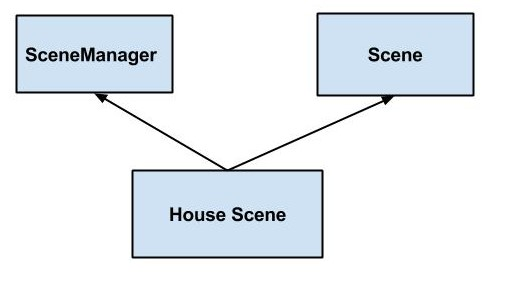
\includegraphics[width=90mm]{images/scenemanager.jpg}
\caption{}
\label{scenemanager}
\end{figure}

SceneManager contains useful tools for the creation, deletion and changing of scenes. The "HomeScene" extends this and contains objects which are all instances of Scene and represent the individual rooms. By extending the SceneManager the HomeScene can listen to events occurring in the game and specify custom ones that are unique for that collection of scenes(or rooms), for example it can specify that doors require changing and loading of different rooms. 

\subsubsection{House implementation}
In addition to remodelling parts of the house a bathroom was created and added along with new actions such as being able to flush the toilet(with sounds to accompany this). Now being able to handle individual objects in rooms allows for easy addition animation, the clock's hands in the room move and will indicate the time of day. Below gives some screen shots of the new environment and it's accompanying frame-rates. 


\begin{figure}[H]
\centering
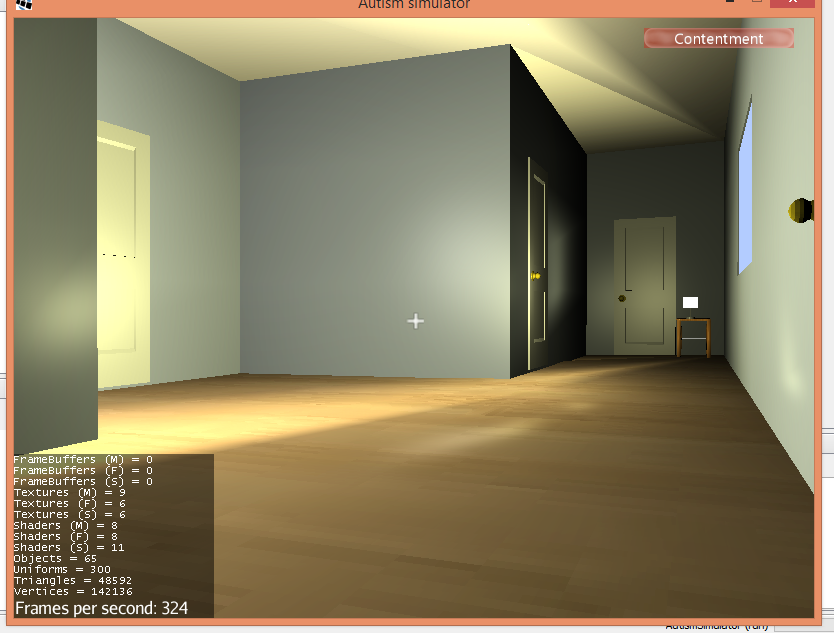
\includegraphics[width=90mm]{images/new_hallway1.png}
\caption{Image of new hallway}
\label{newhallway}
\end{figure}

\begin{figure}[H]
\centering
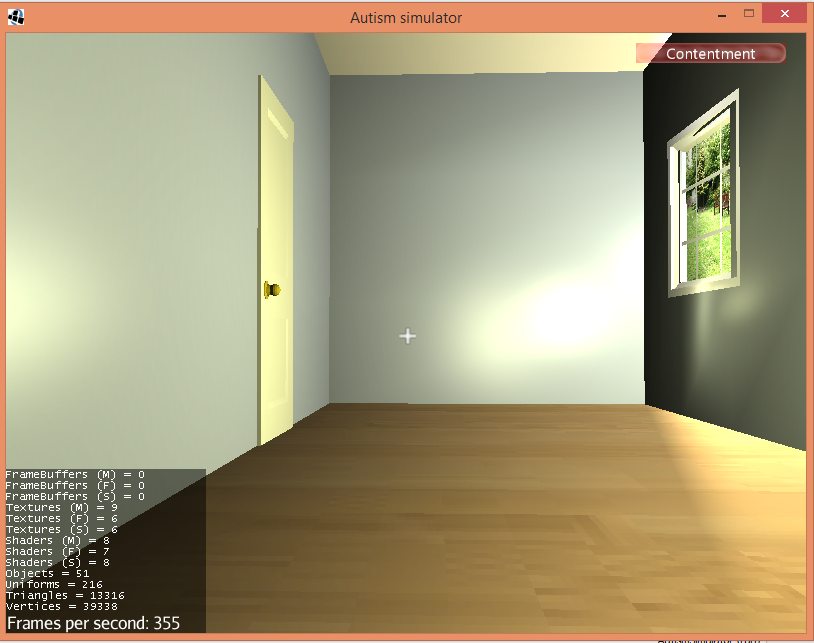
\includegraphics[width=90mm]{images/new_hallway2.png}
\caption{Image of new hallway}
\label{newhallway2}
\end{figure}

\begin{figure}[H]
\centering
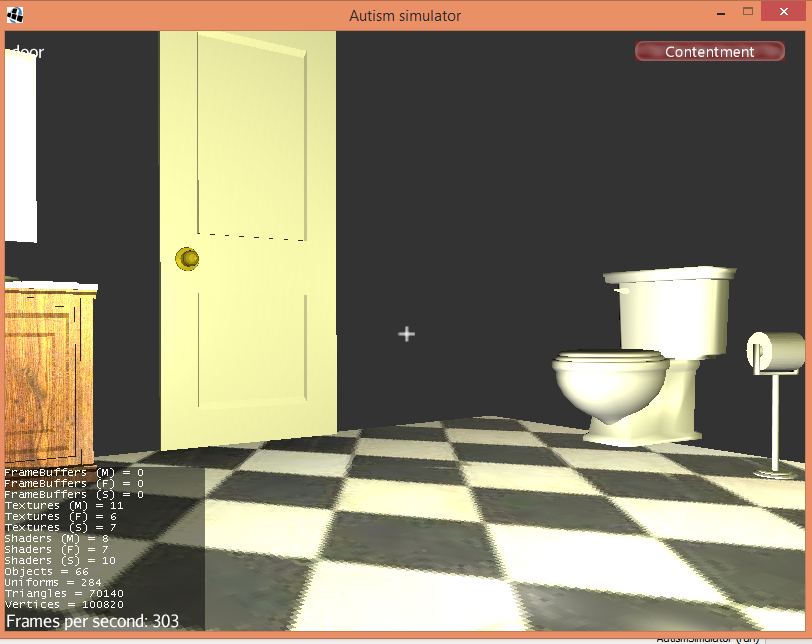
\includegraphics[width=90mm]{images/new_bathroom.png}
\caption{Image of bathroom that was previously missing from the house}
\label{old_house}
\end{figure}

\begin{figure}[H]
\centering
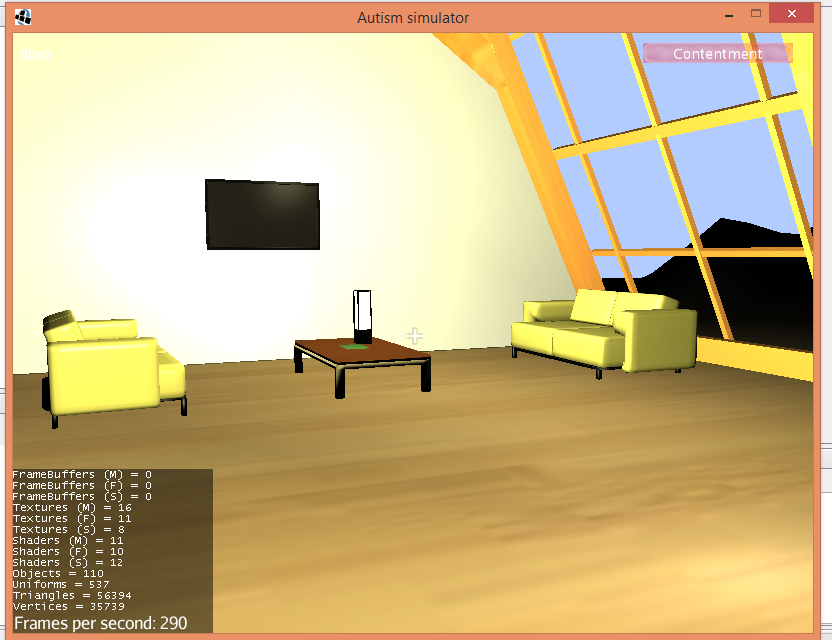
\includegraphics[width=90mm]{images/new_livingroom.png}
\caption{Image of new livingroom}
\label{old_house}
\end{figure}

\subsection{Game state manager}

As the size of the system grew, one of the most important changes was the addition of a game state manager, enabling universal control and monitoring of the overall system. 

The user can now change between "Explore mode"(the user has no tasks and can simply look around the environment) and "Mission mode"(given the tasks or story) without having to restart the simulator. From this came the addition of the start and help screen and ability for the user to pause the game.  

The rest of the system can now request useful information from the GSM such as which mission is currently being run, which scene the player is currently in and what the state of the GUI is (if actions are being displayed, if the user is required to select an option). If the GUI needs to display information(such as selecting actions) it will notify the game state manager which will halt processes that may interfere. Having a central control made other parts of the simulator easier to develop and reuse since each part of the system only needs to worry about which state it is in rather than checking multiple conditions.

\subsection{Sensory System improvements}
Following the feedback on sensory overloads, improvements were required in how sensory overloads occurred rather than what was happening when they did. Previously, objects which could affect the sensory system were put into a Hashable which were then periodically checked for the distance to the player and if in proximity, would affect the sensory system depending on how far the object is. However, all objects would affect the user by the same weight and the effect on contentment would change depending on what threshold of objects were reached (i.e if 2 were in proximity the health reduction would be low, if more than two the reduction would be greater). Filters to mirror sensory overloads would then be applied depending on this level.

\begin{figure}[H]
\centering
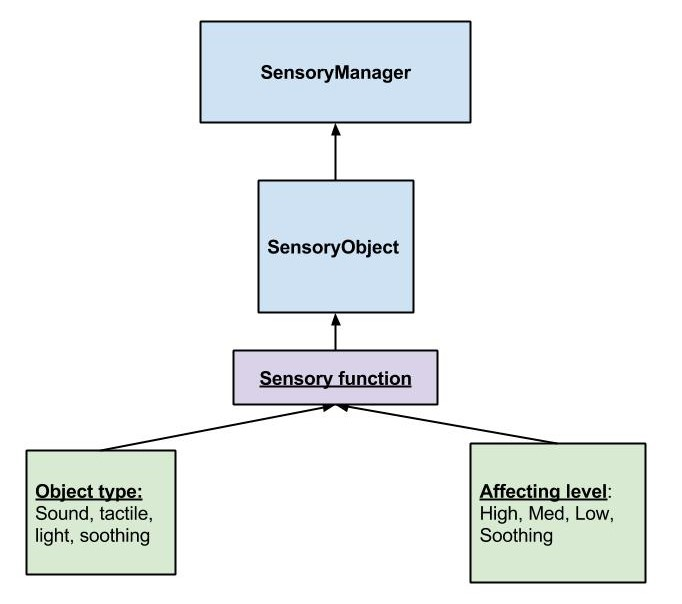
\includegraphics[width=90mm]{images/sensoryobjects.jpg}
\caption{Diagram showing implementation of sensory system}
\label{sensorysystem}
\end{figure}

The new implementation attempts to create a better less fragmented model of how objects affect the player and cause sensory overloads/meltdowns. This approach is more scalable and enables a flexible means to experiment by simply changing parameters, thus helping to address previous issues of meltdowns occurring too quickly.

Each sensory object is given two properties (from the green boxes above) and from this a sensory function is applied and a weight for each object is calculated. The sensory function is simply an exponential: the higher the affecting level the higher the weight returned and if the object is set as a 'soothing object' a negative value will return instead. 

The sensory manager then takes all the weights of the objects that are in proximity and sums them, taking the log of this. If the log is negative there are no objects and contentment replenishes. The result of the summation is then taken away from the players contentment. 

Sounds were the final addition to the simulator. When acting on the toilet it now flushes and the alarm clock in the room rings. Sounds create a more immersive environment and an additional layer for creating sensory overloads(i.e making objects more high-pitched). 

\chapter{First version}

\chapter{Formative evaluation}
- people mentioned that some of the effects were causing them sensory overloads
- Type types. Video for feedback as well as in-person. 
- People who were in the formative evaluation. Need to include Markus and James. Focus on game-play. 
- Video sent out to various people.

\chapter{Summative evaluation}
- Users tended to use different strategies.
- One of the users was deaf, and the message was conveyed to her very accurately. Asked good questions such as "Does this mean if someone with autism comes to visit, I should offer them a quiet room?". 

\chapter{Conclusions}

- response from people, quotes etc. 
- being in a fortunate position of having a supervisor who was well knowledge in the field as well as family members with autism put me in an extremely idea position to build this project. As described in the lit review, it can be very difficult for peopel with autism to explain their problems, thus its very hard to be able to draw conclusions about what to convey.
- multiple evaluations used which was vital. each gave differing information, but even still, more would have been better. 
- big project; it required being a researcher, a creator to represent the varying difficulties, a graphics designer to create the 3d models, an artist for the gui's and images, and a programmer; skills that are usually separate in the game programming industry
- having members of the family with difficulties meant I was aware of how difficult it can be to understand them, no matter how much help and explanation was given. 
- when it was first taken there was a lot of trepidation on whether it was possible given the time restraints, but not only has it proven to be possible; a project has been created where research has shown, albeit unfortunately on the small scale, to be successful in raising knowledge about autism. 
- there was not much research into the success of using simulations to aid understanding of neurological conditions, but this project has shown that visual simulations can aid as a successful tool. 
- depicting sensory overloads and designing and algorithm to do this was extremely difficult. The ere is a vast amount of differing literature on the topic, vast amount of different experiences and even then as people with autism have expressed, sensory differences can be extremely difficult to express. Interviews allowed some insight into this, videos and feedback helped with more, and later feedback given will help develop future improvements. But, still more research is required. There were features from the prototype which are preferred to the first version design such as the delay in sensory overload occurring and delay in coming back to normality. Lights were treated in a better way however by using the first version and getting feedback is was found that the depiction of sounds was extremely accurate. Thus, combining the two preferences on both versions should aid a better result. 
There is still much to be learnt about autism, there is still much research and understanding to acquire, but the tool developed has proven to be useful not only aiding other's understanding of autism and giving an experience which has proven to aid understanding but potentially being used as a platform to aid people with autism being able to explain their difficulties and differences in a less painful way than words. 

\section{Time plan}
- too much time in the first year on pulling things together rather than learning how to use them. This had later repercussions when I had to redo all the scenes and not having forsight of the potential problems involved.

\section{Discussion of tools}
Jmonkey
- offered a lot for importing models
- only really used the scene graph and some other features
- couldn't focus on higher level concepts until the last month of the project
- unity may have been a better choice in regards to being able to focus on that but it wouldn't have allowed the flexibility. It has better model importing. But now I can build and allow others to make their own scenarios
- couldnt focus on higher level until scene rewrite was done which took a good 4 weeks
- didn't use too much of engine. project still ended up being 4k lines of code.
- time spend exploring and learning the different options would have been good
- book for jmonkey didn't come out until december
- doesn't have many ai options
- blender was awesome but should have spent more time at the beginning learning to use the tool rather than focusing on advise to find other models to use. Far too much time was spend on importing and finding suitable models when I could have just created them. Likewise, sketchup was used for this reason which although offered some assistance in the final product no sketchup models were used. It is not idea game asset creation.

\section{Future work}

As the tool created is effectively a platform for more, there are many future possibilities. 
\begin{enumerate}
\item Occulus rift
\item Neurosky portable eeg headset(no, not ridiculous, this is better than it sounds...)
\item Supporting others using system to build their own experiences. This is actually mostly done but would requires better documentation(on the code and on how to create the individual scenarios) and more abstraction if it is required to be obfuscated. Platform needs to be built to aid people developing their own stuffs. 
\item Modelling people with autism and their difficulties and being able to see in what way the world effects them. 
\item Additional stories and scenarios in order to convey other already implemented features such as odd body language. 
\item could be used as a tool for people to use to try out different strategies in environments. 
\end{enumerate}

\chapter{Appendix}

\begin{thebibliography}{9}

\bibliographystyle{plainnat}

\bibitem{increasingprevalence}
Johnny L. Matson, Alison M. Kozlowski
The increasing prevalence of autism spectrum disorders. Research in Autism Spectrum Disorders(2011)

\bibitem{nas}
National autistic society. www.autism.org.uk

\bibitem{statsandfacts}
Ambitious about autism. www.ambitiousaboutautism

\bibitem{nasschool}
Make school make sense. Autism and education: the reality for families today. National Autistic Society, 

\bibitem{autismmisconception}
Autism misconceptions. NHS

\bibitem{olgab}
Sensory Perceptual Issues in Autism and Aspergers syndrome(2003). Bogdeshina, O

\bibitem{fears}
Unusual fears in children with autism(2012). Susan Dickerson Mayes, Susan L. Calhound, Richa Aggarwal, Courtner Baker, Santosh Mathapati, Sarah Molitoris, Rebeccas D. Mayes.

\bibitem{temperament}
Sensory correlates of difficult temperament characteristics in preschool children with autism(2012). I-Ching Chaung, Mei-Hui Tseng, Lu Lu, Jeng-Yi Shieh

\bibitem{bayes}
When the world becomes 'too real': a Bayesian explanation of autistic perception(2012). Elizabeth Pellicano and David Blurr.

\bibitem{williams1996}
Autism: An inside-out approach(1996). Williams, D

\bibitem{williams1994}
Somebody Somewhere: Breaking Free from the World of Autism(1994). Williams, D.

\bibitem{williams1992}
Nobody no-where(1992). Williams, D

\bibitem{sensory_leisure}
Sensory processing abilities and their relation to participation in leisure activities among children with high-functioning autism spectrum disorder. Hochhauser, M. Engel-Yeger, B.

\bibitem{sensory_toddlers}
Parent Reports of Sensory Symptoms in Toddlers with Autism and Those with Other Developmental Disorders. Sally J. Rogers, Susan Hepburn, Elizabeth Wehner

\bibitem{sensory_children}
Describing the sensory abnormalities of children and adults with autism(2007). Susan R. Leekam. Carmen Nieto. Sarah J. Libby. Lorna wing. Judith gould. 

\bibitem{sensory_perceptual}
Sensory integration and the perceptual experience of persons with autism(2006). Grace Iarocci. John McDonald.

\bibitem{rss_cognitive}
Restricted and Repetitive Behaviours, Sensory Processing and Cognitive Style in Children with Autism Spectrum Disorders(2009). Yu-Han Chen, Jacqui Rodgers, Helen McConachie.

\bibitem{rrsyouth}
Restricted and repetitive behaviours and psychiatric symptoms in youth with autism spectrum disorders(2013) Elizabeth A. Stratic, Luc Lecavlier.

\bibitem{rrs_sensory}
Is there a relationship between restricted, repetitive, sterotyped behaviours and interests and abnormal sensory response in children with autism spectrum disorders?(2008). Robin L. Gabriels, John A. Agnew, Lucy Jane Miller, Jane Gralla, Juliet P. Dinkins, Elizabeth Hooks.

\bibitem{aspieway}
"It’s like you are just a spectator in this thing": Experiencing social life the 'aspie' way(2008). Sara Ryan, Ulla Raisanen

\bibitem{dd}
Disability awareness: Beyond the day: http://www.serviceandinclusion.org/index.php?page=simulations. Danielle Dreilinger

\bibitem{autism_awareness}
Awareness and knowledge of autism and autism interventions: A general population survey. Karola Dillenburger(2013). Julie Ann Jordan, Lyn McKerr, Paula Devine, Mickey Keenan

\bibitem{teachersinclusion}
Factors relating to education professionals' classroom practices for the inclusion of students with ASD. Matthew J Segall, Jonathon M. Campbell. 

\bibitem{meltdowns_goingout}
'Meltdowns', surveillance and managing emotions: going out with children with autism(2010). Sara Ryan.

\bibitem{sensory_overview}
Sensory issues in Autism(2007). East sussex county council. 

\bibitem{rss_anxiety}
Relations amoung restricted and repetitive behaviours, anxiety and sensory features in children with autism spectrum disorders(2004)

\bibitem{dsm5}
DSM-5: http://crackingtheenigma.blogspot.co.uk/2014/01/the-evolution-of-autism-comparing-dsm.html

\bibitem{dsm52}
Diagnostic and Statistical Manual of Mental Disorders (DSM-5)

\bibitem{udyslexia}
Understanding dyslexia: http://www.weau.com/home/headlines/Understanding-dyslexia-by-walking-in-their-shoes-199472921.html

\bibitem{dyslexiasimrev}
Virtual Environments and Dyslexia: A literature review(2014), Katerina Kalyvioti*, Tassos A. Mikropoulos 

\bibitem{dyslexicsimpar}
The impact of virtual reality on parent's awareness of cognitive perceptions of a dyslectic child(2008), David Passig, Sigal Eden, Vanina Rosenbaum

\bibitem{sensoryexperiences}
First-hand accounts of sensory perceptual experiences in autism: a qualitative analysis. Robert S P Jones. Ciara Quigney. Jaci C Huws

\bibitem{minshewmodel}
Autism as a Disorder of Complex Information Processing. Nancy J. Minshew and Gerald Goldstein. 

\bibitem{iaroc}
Sensory Integration and the Perceptual Experience of Persons with Autism(2006). Grace Iarocci and John McDonald

\bibitem{teacherchallenge}
Assessing need in school-aged children with an autism spectrum disorder(2010)

\end{thebibliography}

\end{document}